%\documentclass[10pt]{beamer}
%\documentclass{beamer}
\documentclass[handout]{beamer}
\usepackage{ctex}

%\usepackage[orientation=landscape,size=custom,width=16,height=12,scale=0.5,debug]{beamerposter}
 % 1. packages

 % ----------- fonts and symbles ---------
\usepackage{amsmath,amssymb,amsfonts,amsthm}
%\usepackage{CJK}
\usepackage{dsfont}
\usepackage{mathrsfs}
\usepackage{eucal} % for \mathcal

%\renewcommand{\rmdefault}{ptm}


%\usepackage{fontspec}
%\newfontfamily\monaco{Monaco}

%\usepackage{mathbbold} %,bbold

 \usepackage{textcomp} % for \textnormal{\textperthousand}
% -----------------





%\usepackage{slashbox}
%\usepackage[margin=2.2cm]{geometry} % |geometry| package clash with |booktabs| package
%\usepackage{cases}
% -------- tables -------
\usepackage{booktabs} % for \toprule, \bottomrule
\usepackage{tabularx}
\usepackage{multirow}
% --------- figures ---------
\usepackage{graphicx}
% ---------- algorithms -------
\usepackage{algorithm}
\usepackage{algorithmic}
%\usepackage{footnote}
    % |footnote| package occurs error:
    % Runaway argument?
    % \def \insertfootnotetext {\@@ }\def \insertfootnotemark {\@makefnmark \ETC.

\usepackage{listings}

\usepackage[linewidth=1pt]{mdframed} % for  mdframe environment




 \usepackage{color}
 \usepackage{xcolor}     %¸ßÁÁʹÓõÄÑÕÉ«

\usepackage{setspace}
%%\usepackage{type1cm}
\usepackage{adjustbox} % for \adjustbox

\usepackage{accsupp}
\newcommand{\emptyaccsupp}[1]{\BeginAccSupp{ActualText={}}#1\EndAccSupp{}}




%%   figures and tables
\graphicspath{{figure/}}


% 2. new commands

% 2.0 common commands
%\newcommand{\bc}{\begin{center}}
%\newcommand{\ec}{\end{center}}
%\newcommand{\ba}{\begin{array}}
%\newcommand{\ea}{\end{array}}
%\newcommand{\be}{\begin{equation}}
%\newcommand{\ee}{\end{equation}}

% 2.1 colors
\definecolor{dgrey}{rgb}{0.30,0.30,0.30}
\definecolor{lred}{rgb}{0.50,0.00,0.50}
\definecolor{lblue}{rgb}{0.8,0.8,1}
\definecolor{dred}{rgb}{0.6,0,0}
\definecolor{dblue}{rgb}{0,0,0.5}
\definecolor{dgrey}{rgb}{0.35,0.35,0.35}
\definecolor{rred}{rgb}{0.9,0,0}
\definecolor{mylblue}{rgb}{0.3,0.2, 0.8}

\definecolor{commentcolor}{RGB}{85,139,78}
\definecolor{stringcolor}{RGB}{206,145,108}
\definecolor{keywordcolor}{RGB}{34,34,250}
\definecolor{backcolor}{RGB}{220,220,220}

\newcommand{\blue}[1]{{\color{blue}#1}}
\newcommand{\dblue}[1]{{\color{dblue}#1} }
\newcommand{\red}[1]{{\color{red}#1}}
\newcommand{\dred}[1]{{\color{dred}#1}}
\newcommand{\cyan}[1]{{\color{cyan}#1}}
\newcommand{\bfblue}[1]{\textbf{\color{dblue}#1} }
\newcommand{\bfred}[1]{\textbf{\color{dred}#1} }
\newcommand{\green}[1]{{\color{green}#1}}
%\newcommand{\alert}[1]{{\color{red}#1}}
\newcommand{\black}[1]{{\color{black}#1}}
\newcommand{\light}[1]{{\color{blue}\textbf{#1}}}
\newcommand{\hot}[1]{{\color{dred}#1}}
 \newcommand{\highlight}[1]{ \textbf{\color{mylblue}#1}}
 \newcommand{\important}[1]{{\color{red}#1}} % for highlighting  some words

 \newcommand{\mystar}{\dred{$^{\clubsuit}$ }}
  \newcommand{\doublestar}{\dred{$^{\clubsuit\clubsuit}$ }}

\newcommand{\mynote}[1]{{\footnotesize \color{mylblue}#1}}

 \newcommand{\hint}[1]{{\small \color{mylblue}#1}}
\newcommand{\smallhint}[1]{{\small \color{dgrey}#1}}
\newcommand{\footnotehint}[1]{{\footnotesize \color{dgrey}#1}}
\newcommand{\tinyhint}[1]{{\tiny \color{dgrey}#1}}
\newcommand{\mytitle}[1]{\medskip{\large \textbf{\color{mylblue}#1}}}
\newcommand{\normaltitle}[1]{\medskip{ \textbf{\color{mylblue}#1}}}

%\newcommand{\head}[1]{\textbf{\large\color{blue}#1}}
%\newcommand{\heading}[1]{\textbf{\large\color{blue}#1}}

\newcommand{\myfbox}[2]{ \bigskip \begin{center} \fbox{\parbox{#1}{ #2  }} \end{center}\bigskip }

\newcommand{\myvar}[1]{}
%\newcommand{\mynote}[1]{#1}

% 2.2 mathematical symbols

\newcommand{\drightarrow}{\stackrel{d.}{\rightarrow}}
\newcommand{\prightarrow}{\stackrel{p.}{\rightarrow}}
\newcommand{\bernoulli}{\textnormal{Ber}}
\newcommand{\cov}{\mathsf{Cov}}
\newcommand{\corr}{\mathbf{Corr}}
\newcommand{\regret}{\textnormal{Regret}}
\newcommand{\conv}{\textnormal{conv}}
\newcommand{\dotdiv}{\stackrel{\centerdot}{-}}
\newcommand{\dom}{\textnormal{dom}}
\newcommand{\convergenceinprob}{\stackrel{P}{\rightarrow}}
\newcommand{\convergenceindist}{\rightsquigarrow}
\newcommand{\probability}{\mathbb{P}}
\newcommand{\expectation}{\mathbb{E}}
\newcommand{\epi}{\textnormal{epi}}
\newcommand{\variance}{\mathbb{V}}
\newcommand{\var}[1]{\mathbb{V}(#1)}
\newcommand{\covariance}{\mathsf{Cov}}
\newcommand{\empiricalrisk}[1]{\hat{R}(#1)}
\newcommand{\expectedrisk}[1]{R(#1)}
\newcommand{\mgf}[1]{\psi_{#1}(\lambda)}
\newcommand{\mgfexpansion}[1]{\expectation[e^{\lambda#1}]}
\newcommand{\mgfmultivariate}[1]{\expectation[e^{\lambda^\transpose#1}]}
\newcommand{\transpose}{{\mathsf{T}}}
\newcommand{\real}{\mathbb{R}}
\newcommand{\gaussian}[2]{\mathcal{N}(#1,#2)}
\newcommand{\subGaussian}[1]{\mathsf{subG}(#1)}
\newcommand{\indicator}[1]{\mathbb{I}[#1]}
\newcommand{\x}[1]{x^{(#1)}}
\newcommand{\y}[1]{y^{(#1)}}
\newcommand{\z}[1]{z^{(#1)}}
\newcommand{\feature}{x}
\newcommand{\response}{y}
\newcommand{\supofempiricalprocess}{\|\mathbb{P}_n-\mathbb{P}\|_{\decisionspace}}
\newcommand{\decisionspace}{\mathscr{F}}
\newcommand{\decisionfunction}{f}
\newcommand{\featurespace}{\mathcal{X}}
\newcommand{\classifierestimate}{\widehat{h}}
\newcommand{\classifiertrue}{h^\star}
\newcommand{\classifier}{h}
\newcommand{\hypothesisclass}{\mathcal{H}}
\newcommand{\dataset}{\mathcal{D}}
\newcommand{\defineas}{\stackrel{\textnormal{def}}{=}}
\newcommand{\rademachercomplexity}[1]{\mathsf{Rad}_n\left(#1\right)}
\newcommand{\loss}{\ell}
\newcommand{\composite}{\circ}
\newcommand{\convexhull}{\mathsf{conv}}
\newcommand{\norm}[2][2]{\|#2\|_{#1}}
\newcommand{\shatteringcoefficient}[2]{\mathcal{S}(#1,#2)}
\newcommand{\vcdimension}[1]{\mathsf{VC}\left(#1\right)}
\newcommand{\rank}{\mathsf{rank}}
\newcommand{\innerproduct}[2]{\left\langle #1, #2\right\rangle}
\newcommand{\modelparameter}{\theta}
\newcommand{\ball}[3][]{\mathcal{B}_{{#1}}\left(#2,#3\right)}
\newcommand{\metric}{d}
\newcommand{\coveringnumber}[4][]{N_{{#1}}\left(#2,#3,#4\right)}
\newcommand{\trace}{\textnormal{tr}}
\newcommand{\std}{\textnormal{std}}
\newcommand{\sgn}{\textnormal{sign}}
%\renewcommand{\span}{\textnormal{span}}

 % do not overwrite the existing command \span
 % as it leads to an error of
 %  "Missing # Inserted in Alignment Preamble" for ``align'' environment

\newcommand{\myspan}{\textnormal{span}}

%%%
\newcommand{\rightarrowd}{\stackrel{d}{\rightarrow}}
\newcommand{\rightarrowp}{\stackrel{p}{\rightarrow}}
\newcommand{\defeq}{ \stackrel{\textnormal{def}}{=}}
\newcommand{\proj}{ \textnormal{Proj}}
\newcommand{\dist}{\textnormal{dist}}

\newcommand{\argmax}{\textnormal{argmax}}
\newcommand{\argmin}{\textnormal{argmin}}
\newcommand{\subg}{\textnormal{subG}}


 \newcommand{\bba}{\mathbb{A}}
\newcommand{\bbb}{\mathbb{B}}
\newcommand{\bbc}{\mathbb{C}}
\newcommand{\bbd}{\mathbb{D}}
\newcommand{\bbe}{\mathbb{E}}
\newcommand{\bbf}{\mathbb{F}}
\newcommand{\bbg}{\mathbb{G}}
\newcommand{\bbh}{\mathbb{H}}
\newcommand{\bbi}{\mathbb{I}}
\newcommand{\bbj}{\mathbb{J}}
\newcommand{\bbk}{\mathbb{K}}
\newcommand{\bbl}{\mathbb{L}}
\newcommand{\bbm}{\mathbb{M}}
\newcommand{\bbn}{\mathbb{N}}
\newcommand{\bbo}{\mathbb{O}}
\newcommand{\bbp}{\mathbb{P}}
\newcommand{\bbq}{\mathbb{Q}}
\newcommand{\bbr}{\mathbb{R}}
\newcommand{\bbs}{\mathbb{S}}
\newcommand{\bbt}{\mathbb{T}}
\newcommand{\bbu}{\mathbb{U}}
\newcommand{\bbv}{\mathbb{V}}
\newcommand{\bbw}{\mathbb{W}}
\newcommand{\bbx}{\mathbb{X}}
\newcommand{\bby}{\mathbb{Y}}
\newcommand{\bbz}{\mathbb{Z}}

\newcommand{\bfa}{\mathbf{a}}
\newcommand{\bfb}{\mathbf{b}}
\newcommand{\bfc}{\mathbf{c}}
\newcommand{\bfd}{\mathbf{d}}
\newcommand{\bfe}{\mathbf{e}}
\newcommand{\bff}{\mathbf{f}}
\newcommand{\bfg}{\mathbf{g}}
\newcommand{\bfh}{\mathbf{h}}
\newcommand{\bfi}{\mathbf{i}}
\newcommand{\bfj}{\mathbf{j}}
\newcommand{\bfk}{\mathbf{k}}
\newcommand{\bfl}{\mathbf{l}}
\newcommand{\bfm}{\mathbf{m}}
\newcommand{\bfn}{\mathbf{n}}
\newcommand{\bfo}{\mathbf{o}}
\newcommand{\bfp}{\mathbf{p}}
\newcommand{\bfq}{\mathbf{q}}
\newcommand{\bfr}{\mathbf{r}}
\newcommand{\bfs}{\mathbf{s}}
\newcommand{\bft}{\mathbf{t}}
\newcommand{\bfu}{\mathbf{u}}
\newcommand{\bfv}{\mathbf{v}}
\newcommand{\bfw}{\mathbf{w}}
\newcommand{\bfx}{\mathbf{x}}
\newcommand{\bfy}{\mathbf{y}}
\newcommand{\bfz}{\mathbf{z}}

\newcommand{\bfA}{\mathbf{A}}
\newcommand{\bfB}{\mathbf{B}}
\newcommand{\bfC}{\mathbf{C}}
\newcommand{\bfD}{\mathbf{D}}
\newcommand{\bfE}{\mathbf{E}}
\newcommand{\bfF}{\mathbf{F}}
\newcommand{\bfG}{\mathbf{G}}
\newcommand{\bfH}{\mathbf{H}}
\newcommand{\bfI}{\mathbf{I}}
\newcommand{\bfJ}{\mathbf{J}}
\newcommand{\bfK}{\mathbf{K}}
\newcommand{\bfL}{\mathbf{L}}
\newcommand{\bfM}{\mathbf{M}}
\newcommand{\bfN}{\mathbf{N}}
\newcommand{\bfO}{\mathbf{O}}
\newcommand{\bfP}{\mathbf{P}}
\newcommand{\bfQ}{\mathbf{Q}}
\newcommand{\bfR}{\mathbf{R}}
\newcommand{\bfS}{\mathbf{S}}
\newcommand{\bfT}{\mathbf{T}}
\newcommand{\bfU}{\mathbf{U}}
\newcommand{\bfV}{\mathbf{V}}
\newcommand{\bfW}{\mathbf{W}}
\newcommand{\bfX}{\mathbf{X}}
\newcommand{\bfY}{\mathbf{Y}}
\newcommand{\bfZ}{\mathbf{Z}}


\newcommand{\bfSigma}{\mathbf{\Sigma}}
\newcommand{\bfrho}{\mathbf{\rho}}

\newcommand{\cala}{\mathcal{A}}
\newcommand{\calb}{\mathcal{B}}
\newcommand{\calc}{\mathcal{C}}
\newcommand{\cald}{\mathcal{D}}
\newcommand{\cale}{\mathcal{E}}
\newcommand{\calf}{\mathcal{F}}
\newcommand{\calg}{\mathcal{G}}
\newcommand{\calh}{\mathcal{H}}
\newcommand{\cali}{\mathcal{I}}
\newcommand{\calj}{\mathcal{J}}
\newcommand{\calk}{\mathcal{K}}
\newcommand{\call}{\mathcal{L}}
\newcommand{\calm}{\mathcal{M}}
\newcommand{\caln}{\mathcal{N}}
\newcommand{\calo}{\mathcal{O}}
\newcommand{\calp}{\mathcal{P}}
\newcommand{\calq}{\mathcal{Q}}
\newcommand{\calr}{\mathcal{R}}
\newcommand{\cals}{\mathcal{S}}
\newcommand{\calt}{\mathcal{T}}
\newcommand{\calu}{\mathcal{U}}
\newcommand{\calv}{\mathcal{V}}
\newcommand{\calw}{\mathcal{W}}
\newcommand{\calx}{\mathcal{X}}
\newcommand{\caly}{\mathcal{Y}}
\newcommand{\calz}{\mathcal{Z}}


% 3. theorem and environments

%\newtheorem{theorem}{Theorem}%[section]
\newtheorem{proposition}{Proposition}%[section]
%\newtheorem{property}{Property}%[section]
%\newtheorem{lemma}{Lemma}%[section]
%\newtheorem{corollary}{Corollary}%[section]
%\newtheorem{definition}{Definition}%[section]
%\newtheorem{example}{Example}%[section]
%\newtheorem{remark}{Remark}%[section]
%\newtheorem{note}{Note}%[section]
%\newtheorem{problem}{Problem}%[section]
\newtheorem{exercise}{Exercise}
%\newtheorem{assumption}{Assumption}
\newtheorem*{lemma_star}{Lemma}
\newtheorem*{theorem_star}{Theorem}

%\newenvironment{summary}[1][Summary]{\par\medskip   \color{dred}\textbf{\large#1. } }{ \medskip}
%\newenvironment{remark}[1][Remark]{\par\medskip  \begin{small} \color{dblue}\textbf{#1. } }{ \end{small}\medskip}
%\renewenvironment{proof}[1][Proof]{\noindent\textbf{#1.} }{\mbox{} \hfill{\small\textrm{$\Box$}}\vspace{1ex}}
% \newenvironment{answer}[1][Answer]{\par\medskip \color{dblue}\textbf{\large#1. }}{ \medskip}

\newenvironment{summary}[1][总结]{\par\medskip   \color{dred}\textbf{\large#1 } }{ \medskip}
\newenvironment{remark}[1][注意]{\par\medskip   \color{dblue}\textbf{\large#1 } }{ \medskip}
\newenvironment{footnoteremark}{ \color{dblue}\begin{footnotesize} }{\end{footnotesize}}
\renewenvironment{proof}[1][证明]{\noindent\textbf{#1.} }{\mbox{} \hfill{\small\textrm{$\Box$}}\vspace{1ex}}
 \newenvironment{question}[1][Q.]{\par\medskip {\color{lred}\large#1}}{ \medskip}
 \newenvironment{answer}[1][Answer]{\par\medskip \color{dblue}\textbf{\large#1 }}{ \medskip}

% 4. beamer setting




%\newtheorem{definition}{\textbf{¶¨Òå}}[section]
%\newtheorem{proposition}[definition] { \textbf{ÃüÌâ}}
%\newtheorem{lemma}[definition] { \textbf{ÒýÀí}}
%\newtheorem{theorem}[definition]{ \textbf{¶¨Àí}}
%\newtheorem{corollary}[definition] { \textbf{ÍÆÂÛ}}
%\newtheorem{remark}[definition] { \textbf{×¢}}
%\newtheorem{example}[definition] { \textbf{Àý}}

%\newcommand{\shadow}[1]{\begin{center}
%\bf{\textcolor{dblue}{\shadowbox{\parbox{3.8in}
% {\textcolor{red}
% {\vspace{1mm}#1}}}}}
%\end{center}}
%
%\newcommand{\head}[1]{\begin{center}
%\bf{\textcolor{dblue}{\shadowbox{\parbox{3.8in}
% {\textcolor{dred}
% {\vspace{1mm}#1}}}}}
%\end{center}}
%
%
%\newcommand{\heading}[1]{%
%  \begin{center}
%    \large\bf
%    \shadowbox{#1}%
%  \end{center}
%\vspace{1ex minus 1ex}}

% set  space above and below math equations in display style

\expandafter\def\expandafter\normalsize\expandafter{%
    \normalsize
    \setlength\abovedisplayskip{1.5ex}
    \setlength\belowdisplayskip{1.2ex}
    \setlength\abovedisplayshortskip{0.5ex}
    \setlength\belowdisplayshortskip{0.5ex}
}

% Ìí¼ÓÒ³Âë´úÂ룬¹È¸èÕÒµ½µÄ¡£
\addtobeamertemplate{navigation symbols}{}{%
    %\usebeamerfont{footline}%
    %\usebeamercolor[fg]{footline}%
    \setbeamercolor{footline}{fg=blue}
    \setbeamerfont{footline}{series=\bfseries}
    \hspace{1em}%
    \normalsize{\insertframenumber/\inserttotalframenumber}
}

% section numbering
\setbeamertemplate{section in toc}[sections numbered]
\setbeamertemplate{subsection in toc}[subsections numbered]



\lstset{                        %¸ßÁÁ´úÂëÉèÖÃ
%basicstyle=\small, % print whole listing small
%basicstyle=\footnotesize\sffamily, % print whole listing small
basicstyle=\footnotesize\rmfamily, % print whole listing small
%basicstyle=\rmfamily, % print whole listing small
    language=python,                    %PythonÓï·¨¸ßÁÁ
    %linewidth=0.9\linewidth,            %Áбílist¿í¶È
    %basicstyle=\ttfamily,              %ttÎÞ·¨ÏÔʾ¿Õ¸ñ
    commentstyle=\color{commentcolor},  %×¢ÊÍÑÕÉ«
    keywordstyle=\color{keywordcolor},  %¹Ø¼ü´ÊÑÕÉ«
    stringstyle=\color{stringcolor},    %×Ö·û´®ÑÕÉ«
    %showspaces=true,                   %ÏÔʾ¿Õ¸ñ
    numbers=left,                       %ÐÐÊýÏÔʾÔÚ×ó²à
    %numberstyle=\tiny\emptyaccsupp,     %ÐÐÊýÊý×Ö¸ñʽ
    numberstyle=\tiny,                  %ÐÐÊýÊý×Ö¸ñʽ
    numbersep=5pt,                      %Êý×Ö¼ä¸ô
    frame=single,                       %¼Ó¿ò
    framerule=0pt,                      %²»»®Ïß
    %escapeinside=@@,                    %ÌÓÒݱêÖ¾
    escapeinside=``,                    %ÌÓÒݱêÖ¾
    emptylines=1,                       %
    xleftmargin=3em,                    %list×ó±ß¾à
    backgroundcolor=\color{backcolor},  %ÁÐ±í±³¾°É«
    tabsize=4,                          %ÖƱí·û³¤¶ÈΪ4¸ö×Ö·û
    %gobble=4                            %ºöÂÔÿÐдúÂëÇ°4¸ö×Ö·û
    breaklines=true,
    extendedchars=false
    }

\lstdefinestyle{numbers}{numbers=left, stepnumber=1, numberstyle=\tiny, numbersep=10pt}
 \lstdefinestyle{nonumbers}{numbers=none}

\newcommand{\alertcode}[1]{{\color{red}#1}} % used for alerting codes

%\lstset{numbers=left, numberstyle=\tiny,
%keywordstyle=\color{blue!70},
%commentstyle=\color{red!50!green!50!blue!50},
%frame=shadowbox,
%rulesepcolor=\color{red!20!green!20!blue!20},
%escapeinside=``,
%framesep = 2ex,
%rulesep = 1ex
%%framexrightmargin= 1em %
%}


% Vary the color applet  (try out your own if you like)
\colorlet{structure}{red!65!black}

%\beamertemplateshadingbackground{yellow!50}{white}


%\setbeamerfont{normal text}{family=\rmfamily}
%\setbeamerfont{frametitle}{family=\rmfamily}

% Changing the fonts: this will make the slides more readable and the math look like regular tex math
\usefonttheme{serif}



% set spaces

\setstretch{1.2}  % ÉèÖÃÐоà

\addtobeamertemplate{block begin}{\setlength\abovedisplayskip{0pt}} % reduce the large space before a block

% set section number styles



\newcommand{\secno}{Sec.\,\thesection\ }
\newcommand{\subsecno}{Sec.\,\thesubsection\ }

% set logo

 \pgfdeclareimage[width=1.0]{small-logo}{SMaLL.jpg}
%
 \logo{\vbox{\vskip0.1 \hbox{\pgfuseimage{small-logo}}}}

% set math equation fontsize

 \makeatletter
\DeclareMathSizes{\f@size}{10}{5}{5}
\makeatother

% for chinese section name
\hypersetup{CJKbookmarks=true}


%\usepackage{hyperref}
%\hypersetup{hidelinks,
%	colorlinks=true,
%	allcolors=black,
%	pdfstartview=Fit,
%	breaklinks=true}

\hypersetup{CJKbookmarks=true}
%\newtheorem{example}{Example}%[section]

\newcommand{\zixue}{\hint{(自学)}}	

\begin{document}
	
	\lstdefinestyle{nonumbers}{numbers=none}
	
	\addtobeamertemplate{block begin}{\setlength\abovedisplayskip{0pt}}
	
	\setbeamertemplate{itemize items}{\color{black}$\bullet$}
	
	\title[最优化模型与算法]{第3章\,凸优化模型}
	
	\bigskip
	
	\author[]{
		\underline{SMaLL} 
	}
	
	\institute[CUP]{
		\inst{1}
		中国石油大学(华东)\\
		SMaLL 课题组   \\
		\blue{small.sem.upc.edu.cn}\\
		liangxijunsd@163.com \\ 
		
	}
	
	\date[2023]{\small    2023}
	
	\subject{convex optimization}
	
	\frame{\titlepage}
	
	
	
	%\frame{
		%	\frametitle{}
		%	\tableofcontents[hideallsubsections]
		%}
	
	
	\setcounter{section}{4}
	
	\AtBeginSection[]{
		\begin{frame}
			\frametitle{}
			\tableofcontents[currentsection,currentsubsection]
		\end{frame}
	}
	
	\AtBeginSubsection[]{                              % 在每个Section前都会加入的Frame
		%\frame<handout:1>{
			\begin{frame}
				\frametitle{ }
				\tableofcontents[current,currentsubsection] % 显示在目录中加亮的当前章节
				%\tableofcontents[hideallsubsections,currentsection] % 显示在目录中加亮的当前章节
				%\tableofcontents[current,hideallsubsections]
			\end{frame}
			
			%}
	}
	
	\section{凸优化问题}
	
	\begin{frame}
		\frametitle{本章要点}
		
		\begin{itemize}
			\item 掌握凸优化问题的形式,能够识别凸优化问题
			\item 了解拟凸优化的形式
			\item 掌握线性规划和二次规划的形式,
			能够识别这两类优化问题,并能够调用软件包 解决问题
			
			\item 掌握二阶锥规划 和 半定规划(semidefinite prog.) 的 
			的形式, 
			能够识别这两类优化问题,并能够调用软件包 解决问题
		\end{itemize}
	\end{frame}
	%==============================================================
	%\begin{frame}
	%\begin{large}
	%\centerline{\textbf{4.凸优化问题}}
	%\end{large}
	%\bigskip
	%\bigskip
	%\begin{itemize}
	%	\item 标准形式的优化问题
	%	\bigskip
	%	\item 凸优化问题
	%	\bigskip
	%	\item 拟凸优化
	%	\bigskip
	%	\item 线性规划
	%	\bigskip
	%	\item 二次优化
	%	\bigskip
	%	\item 几何规划
	%	\bigskip
	%	\item 广义不等式约束
	%	\bigskip
	%	\item 半定规划
	%	
	%\end{itemize}
	%\end{frame}
	%===============================================================
	
	
	\subsection{标准形式的优化问题}
	\begin{frame}
		\frametitle{标准形式的优化问题}
		\begin{equation}
			\begin{array}{ll}
				\text{minimize} & f_{0}(x) \\
				\text { subject to } & f_{i}(x) \leq 0, \quad i=1, \ldots, m \\
				& h_{i}(x)=0, \quad i=1, \ldots, p
			\end{array}
		\end{equation}
		\onslide<1->{
			\begin{itemize}
				\item $x \in \mathbb{R}^{n}$ 是优化变量
				\item $f_{0}: \mathbb{R}^{n} \rightarrow \mathbb{R}$ 是目标函数或代价函数
				\item $f_{i}: \mathbb{R}^{n} \rightarrow \mathbb{R}, i=1, \ldots, m,$ 是不等式约束函数
				\item $h_{i}: \mathbb{R}^{n} \rightarrow \mathbb{R}$ 是等式约束函数
			\end{itemize}}
	\end{frame}
		
		\begin{frame}{隐式约束}
			\begin{equation}
				x \in \mathcal{D}=\bigcap_{i=0}^{m} \mathbf{ dom }\ f_{i}\ \cap \ \bigcap_{i=1}^{p} \mathbf{ dom }\ h_{i},
			\end{equation}
			\begin{itemize}[<+->]
				\item 我们称 $\mathcal{D}$ 为问题的\textbf{定义域} 
				\item 约束 $f_{i}(x) \leq 0, h_{i}(x)=0$ 是显式约束
				\item  如果一个问题没有明确的约束 $(m=p=0)$,它就是\textbf{不受约束的}
			\end{itemize}
				\onslide<4->{
				\highlight{ 例.}
					\begin{equation}
						\text { minimize } \quad f_{0}(x)=-\sum_{i=1}^{k} \log \left(b_{i}-a_{i}^{T} x\right)
					\end{equation}
					是一个具有隐式约束$a_{i}^{T} x<b_{i}$的无约束问题
			 }

	
		\end{frame}
		%-------------------------------------------------------
		\begin{frame}[fragile]
			\frametitle{最优点和局部最优点}
			\onslide<1->{
			\highlight{ 定义.}
				如果$x \in \textbf{dom}\ f_{0}$ 并且满足约束条件,则称$x$ 是 \textbf{可行的}\\
			}
				\onslide<2->{ 
					\textbf{最优值p*:}
					\begin{equation}
						p^{\star}=\inf \left\{f_{0}(x) \mid f_{i}(x) \leq 0, i=1, \ldots, m, h_{i}(x)=0, i=1, \ldots, p\right\}
					\end{equation}
				}
				\onslide<3->{
					如果 $f_{0}(x)=p^{\star} $称这个可行的$x$ 为 \textbf{最优解} ; $X_{\text {opt}}$ 是所有最优解的集合\\
				}
				\onslide<4->{
					$x$ 是 \textbf{局部最优的} 如果 存在 $R>0$ 使得 $x$ 是下面关于$z$ 优化问题的解
					\begin{equation}
						\begin{array}{ll}
							\text { minimize (over } z) & f_{0}(z) \\
							\text { subject to } & f_{i}(z) \leq 0, \quad i=1, \ldots, m, \quad h_{i}(z)=0, \quad i=1, \ldots, p \\
							& \|z-x\|_{2} \leq R
						\end{array}
					\end{equation}\\
				}
					\end{frame}
		
		\begin{frame}
				\onslide<4->{
				\highlight{ 例.}	( $n=1, m=p=0$)
					\begin{itemize}%[<+->]
						\item $f_{0}(x)=1 / x,\ \textbf{dom}\ f_{0}=\mathbb{R}_{++}: p^{\star}=0,$ 无最优点
						\item $f_{0}(x)=-\log x,\ \textbf{dom}\ f_{0}=\mathbb{R}_{++}: p^{\star}=-\infty$
						\item $f_{0}(x)=x \log x,\ \textbf{dom}\ f_{0}=\mathbb{R}_{++}: p^{\star}=-1 / e, x=1 / e$ 是最优点
						\item $f_{0}(x)=x^{3}-3 x,\ p^{\star}=-\infty,$ 在$x=1$处局部最优
					\end{itemize}
			
			}
		\end{frame}
	
	%-------------------------------------------------------
	\begin{frame}
		\frametitle{可行性问题}
		\begin{equation}
			\begin{array}{ll}
				\text { find } & x \\
				\text { subject to } & f_{i}(x) \leq 0, \quad i=1, \ldots, m \\
				& h_{i}(x)=0, \quad i=1, \ldots, p
			\end{array}
		\end{equation}\\
		\onslide<2->{	
			当 $f_{0}(x)=0$时,可以认为是一般问题的特例:\\
		}
		\onslide<3->{	
			\begin{equation}
				\begin{array}{ll}
					\text { minimize } & 0 \\
					\text { subject to } & f_{i}(x) \leq 0, \quad i=1, \ldots, m \\
					& h_{i}(x)=0, \quad i=1, \ldots, p
				\end{array}
			\end{equation}
		}
		\onslide<4->{
			\begin{itemize}[<+->]
				\item 如果约束条件可行,那么$p^{\star}=0$ ;任何可行的 $x$ 都是最佳的
				
				\item 如果约束不可行,那么$p^{\star}=\infty$ 
			\end{itemize}
		}
	\end{frame}
	%===============================================================
	\subsection{凸优化问题}
	\begin{frame}
		\frametitle{凸优化问题}
		\textbf{标准形式的凸优化问题}
		\begin{equation}
			\begin{array}{ll}
				\text{ minimize } & f_{0}(x) \\
				\text { subject to } & f_{i}(x) \leq 0, \quad i=1, \ldots, m \\
				& a_{i}^{T} x=b_{i}, \quad i=1, \ldots, p
			\end{array}
		\end{equation}
		\onslide<2->{
			\begin{itemize}[<+->]
				\item
				\dred{$f_{0}, f_{1}, \ldots, f_{m}$ 均为凸函数; 等式约束是仿射函数}
				%\item problem is quasiconvex if $f_{0}$ is quasiconvex (and $f_{1}, \ldots, f_{m}$ convex)
			\end{itemize}
		}	
		
		\onslide<3->{
			重要性质:凸优化问题的可行集是凸的
		}
	\end{frame}
	
	
	
	%--------------------------------------------------------
	\begin{frame}
		\frametitle{示例}
		
		\hint{凸优化问题}
		
		\begin{equation}
			\begin{array}{ll}
				\text{ minimize } & f_{0}(x)=x_{1}^{2}+x_{2}^{2} \\
				\text { subject to } & f_{1}(x)=x_{1} /\left(1+x_{2}^{2}\right) \leq 0 \\
				& h_{1}(x)=\left(x_{1}+x_{2}\right)^{2}=0
			\end{array}
		\end{equation}\\
		\begin{itemize}[<+->]
			\item  $f_{0}$ 是凸函数; 可行集$\left\{\left(x_{1}, x_{2}\right) \mid x_{1}=-x_{2} \leq 0\right\}$ 是凸集
			
			\item (根据我们的定义)并非一个凸优化问题: $f_{1}$ 不是凸函数, $h_{1}$ 不是仿射函数
			
			\item 与凸问题等价(但不相同)
			\begin{equation}
				\begin{array}{ll}
					\text { minimize } & x_{1}^{2}+x_{2}^{2} \\
					\text { subject to } & x_{1} \leq 0 \\
					& x_{1}+x_{2}=0
				\end{array}
			\end{equation}
		\end{itemize}
	\end{frame}
	%------------------------------------------------------
	\begin{frame}
		\frametitle{局部和全局最优}
		\begin{theorem}
			凸问题的任何局部最优点都是(全局)最优的\\
		\end{theorem}
		\onslide<2->{
			\begin{proof}假设 $x$ 是局部最优的,但存在一个可行的 $y$ ,$f_{0}(y)<f_{0}(x)$\\
				
				$x$ 局部最优意味着存在$R>0$ 使得
				\begin{equation}
					z \text { 可行, } \quad\|z-x\|_{2} \leq R \quad \Longrightarrow \quad f_{0}(z) \geq f_{0}(x)
				\end{equation}\\
			}
			\onslide<3->{
				令 $z=\theta y+(1-\theta) x$ ,其中 $\theta=R /\left(2\|y-x\|_{2}\right)$\\
				\begin{itemize}[<+->]
					\item $\|y-x\|_{2}>R,$ 所以 $0<\theta<1 / 2$
					\item $z$ 是两个可行点的凸组合,因此也是可行的
					\item $\|z-x\|_{2}=R / 2$ 且
					\begin{equation}
						f_{0}(z) \leq \theta f_{0}(y)+(1-\theta) f_{0}(x)<f_{0}(x)
					\end{equation}
					这与我们的假设相悖,即 $x$ 是局部最优的
				\end{itemize}
			\end{proof}
		}
	\end{frame}
	%--------------------------------------------------------
	\begin{frame}
		\frametitle{可微函数$f_0$的最优性准则}
		\begin{theorem}
			对于任何凸优化问题,$x$是最优的,当且仅当其可行且
			\begin{equation}
				\nabla f_{0}(x)^{T}(y-x) \geq 0 \quad \text{对所有可行}\ y
			\end{equation}
		\end{theorem}
		\only<2-3>{
			\begin{figure}
				\centering
				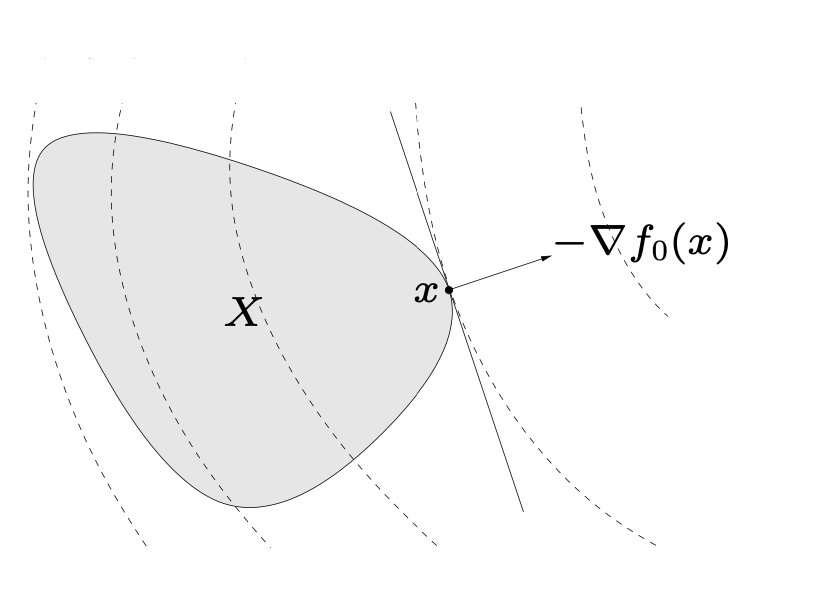
\includegraphics[width=0.5\textwidth]{Ch4-Optimality-criterion-for-differentiable}
			\end{figure}
		}
		\only<3-3>{
			其中可行集x由阴影表示,如果非零, $\nabla f_{0}(x)$ 在$x$处定义了可行集 $X$的一个支撑超平面
		}
	\end{frame}
	
	\begin{frame}
		
		\frametitle{证明.}
		
		证明.
		\only<1-2>{
			$\Longleftarrow$: $f_0$ 为凸函数: $ f_0(y) \geq f_0(x) + \langle \nabla f_0(x), y-x \rangle $,
			$\forall x,y \in \textnormal{dom}\, f_0$
		}
		
		\only<2-2>{
			$\Longrightarrow$:
			假设 $x$ 是最优的, $\exists y\in X$,满足
			$   \langle \nabla f_0(x), y-x \rangle <0$.
			
			考虑点  $z(t)=t y+(1-t) x$, 其中 $t \in[0,1]$.
			$X$ 是凸集 $\Rightarrow$ $z(t)$ 是可行的.
			
			对于较小的正数 $t$: $f_{0}(z(t))<f_{0}(x)$,
			$\Rightarrow$ $x$ 不是最优的.
			为了说明这点:
			$$
			\left.\frac{d}{d t} f_{0}(z(t))\right|_{t=0}=\nabla f_{0}(x)^{T}(y-x)<0
			$$
			对于较小的正数 $t$: $f_{0}(z(t))<f_{0}(x)$.
		}
		
	\end{frame}
	
	
	
	
	
	%-------------------------------------------------------
	\begin{frame}
		\frametitle{可微函数 $f_0$ 的最优性准则}
		\begin{itemize}[<+->]
			\item \textbf{无约束问题:} $x$ 是最优解,当且仅当
			\begin{equation}
				x \in \textbf{dom}\ f_{0}, \quad \nabla f_{0}(x)=0
			\end{equation}
			\item \textbf{等式约束问题}
			\begin{equation}
				\begin{array}{cc}
					\text { minimize } & f_{0}(x) \quad \text { subject to } \quad A x=b
				\end{array}
			\end{equation}
			$x$ 是最优解,当且仅当 存在一个 $\nu$ 使得
			\begin{equation}
				x \in \textbf{dom}\ f_{0}, \quad A x=b, \quad \nabla f_{0}(x)+A^{T} \nu=0
			\end{equation}
			\item \textbf{非负整数的最小化}
			\begin{equation}
				\text{ minimize } \quad f_{0}(x) \quad \text{subject to} \quad x \succeq 0
			\end{equation}
			$x$ 是最优解,当且仅当
			\begin{equation}
				x \in \textbf{dom}\ f_{0}, \quad x \succeq 0, \quad\left\{\begin{array}{ll}
					\nabla f_{0}(x)_{i} \geq 0 & x_{i}=0 \\
					\nabla f_{0}(x)_{i}=0 & x_{i}>0
				\end{array}\right.
			\end{equation}
		\end{itemize}
	\end{frame}
	%-------------------------------------------------------
	\begin{frame}
		\frametitle{等价凸问题}
		如果一个问题的解很容易从另一个问题中得到,则两个问题 (非正式地)是 \textbf{等价的} , 反之亦然\\
		
		\onslide<2->{
			保持凸性的一些常见变换:
		}
		\onslide<3->{
			\begin{itemize}
				\item \textbf{消除等式约束}
				\begin{equation}
					\begin{array}{ll}
						\text{ minimize } & f_{0}(x) \\
						\text { subject to } & f_{i}(x) \leq 0, \quad i=1, \ldots, m \\
						& A x=b
					\end{array}
				\end{equation}
			}
			\onslide<4->{
				等价于
				\begin{equation}
					\begin{array}{ll}
						\text { minimize (over} z) & f_{0}\left(F z+x_{0}\right) \\
						\text { subject to } & f_{i}\left(F z+x_{0}\right) \leq 0, \quad i=1, \ldots, m
					\end{array}
				\end{equation}
				
				其中$F$ 和 $x_{0}$ 满足
				\begin{equation}
					A x=b \quad \Longleftrightarrow \quad x=F z+x_{0} \text {(对一切 } z)
				\end{equation}
			\end{itemize}
		}
	\end{frame}
	%-------------------------------------------------------
	\begin{frame}
		\frametitle{等价凸问题}
		\begin{itemize}[<+->]
			\item \textbf{引入等式约束}
			\begin{equation}
				\begin{array}{ll}
					\text{ minimize } & f_{0}\left(A_{0} x+b_{0}\right) \\
					\text { subject to } & f_{i}\left(A_{i} x+b_{i}\right) \leq 0, \quad i=1, \ldots, m
				\end{array}
			\end{equation}
			等价于
			\begin{equation}
				\begin{array}{ll}
					\text { minimize (over } \left.x, y_{i}\right) & f_{0}\left(y_{0}\right) \\
					\text { subject to } & f_{i}\left(y_{i}\right) \leq 0, \quad i=1, \ldots, m \\
					& y_{i}=A_{i} x+b_{i}, \quad i=0,1, \ldots, m
				\end{array}
			\end{equation}
			
			\item \textbf{引入线性不等式的松弛变量}
			\begin{equation}
				\begin{array}{ll}
					\text { minimize } & f_{0}(x) \\
					\text { subject to } & a_{i}^{T} x \leq b_{i}, \quad i=1, \ldots, m
				\end{array}
			\end{equation}
			等价于
			\begin{equation}
				\begin{array}{ll}
					\text { minimize (over } x, s) & f_{0}(x) \\
					\text { subject to } & a_{i}^{T} x+s_{i}=b_{i}, \quad i=1, \ldots, m \\
					& s_{i} \geq 0, \quad i=1, \ldots m
				\end{array}
			\end{equation}
		\end{itemize}
	\end{frame}
	%-------------------------------------------------------
	\begin{frame}
		\frametitle{等价凸问题}
		\begin{itemize}
			\item \textbf{上图(epigraph)形式:} 标准形式凸问题等价于
			\begin{equation}
				\begin{array}{ll}
					\text{ minimize }(\text {over}\ x, t) & t \\
					\text { subject to } & f_{0}(x)-t \leq 0 \\
					& f_{i}(x) \leq 0, \quad i=1, \ldots, m \\
					& A x=b
				\end{array}
			\end{equation}\\
		\end{itemize}
		\onslide<2->{
			\begin{itemize}
				\item \textbf{最小化某些变量}
				\begin{equation}
					\begin{array}{ll}
						\text{ minimize } & f_{0}\left(x_{1}, x_{2}\right) \\
						\text { subject to } & f_{i}\left(x_{1}\right) \leq 0, \quad i=1, \ldots, m
					\end{array}
				\end{equation}
				等价于
				\begin{equation}
					\begin{array}{ll}
						\text{ minimize } \quad \tilde{f}_{0}\left(x_{1}\right) \\
						\text { subject to } \quad f_{i}\left(x_{1}\right) \leq 0, \quad i=1, \ldots, m
					\end{array}
				\end{equation}
				其中 $\tilde{f}_{0}\left(x_{1}\right)=\inf _{x_{2}} f_{0}\left(x_{1}, x_{2}\right)$
			\end{itemize}
		}
	\end{frame}
	%================================================================
	\iffalse
	\subsection{拟凸优化}
	\begin{frame}
		\frametitle{拟凸优化}
		\begin{equation}
			\begin{array}{ll}
				\text{ minimize } & f_{0}(x) \\
				\text { subject to } & f_{i}(x) \leq 0, \quad i=1, \ldots, m \\
				& A x=b
			\end{array}
		\end{equation}
		$f_{0}: \mathbb{R}^{n} \rightarrow \mathbb{R}$ 为拟凸函数, $f_{1}, \ldots, f_{m}$ 为凸函数\\
		
		
		\onslide<2->{
			可以具有非(全局)最优的局部最优点
		}
		\onslide<3->{
			\begin{figure}
				\centering
				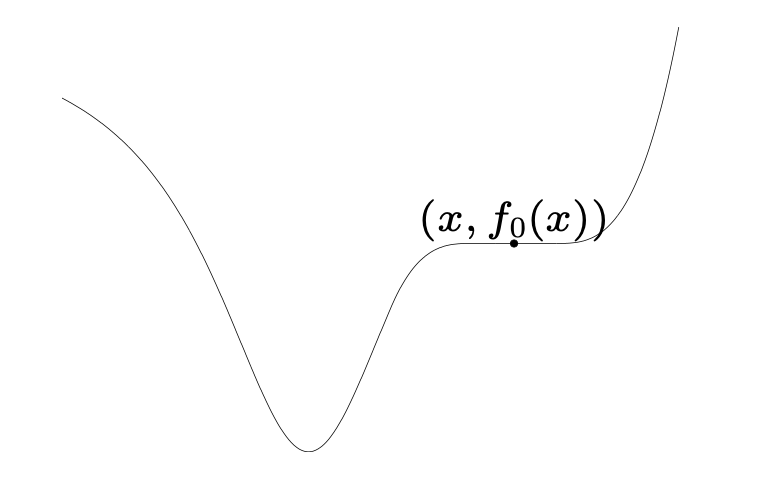
\includegraphics[height=5cm,width=6cm]{Ch4-Quasiconvex-optimization}	
			\end{figure}
		}
    end{frame}
	
	
	
	\begin{frame}
		\frametitle{拟凸优化问题}
		
		\begin{itemize}%[<+->]
			
			\item 如果 $f_{0}$ 是拟凸函数 ( $f_{1}, \ldots, f_{m}$ 为凸函数),那么该问题是拟凸优化问题
		\end{itemize}
		
		\onslide<2->{
			通常写为:
			\begin{equation}
				\begin{array}{ll}
					\text{minimize} & f_{0}(x) \\
					\text { subject to } & f_{i}(x) \leq 0, \quad i=1, \ldots, m \\
					& A x=b
				\end{array}
			\end{equation}
		}
		
		\onslide<3->{
				\highlight{ 定义.}
				[拟凸函数] 函数$f: \mathbb{R}^n \rightarrow \mathbb{R}$
				称为拟凸(或单峰),如果其定义域及所有下水平集
				$$
				S_{\alpha} = \{x\in \dom f \,|\, f(x) \leq \alpha\}
				$$
				对任意 $\alpha \in \mathbb{R}$ 都是凸集.		
		}
		
		
		
	\end{frame}
	
	\begin{frame}
		\onslide<1->{
			\highlight{ 例.}(拟凸函数)
		\begin{itemize}
			\item $\log x$ 在 $\mathbb{R}_{++}$上;
			\item 指数平方损失: $\phi(t) = 1-e^{-\frac{-t^2}{\gamma}}$, $\gamma>0$;
			\item SCAD 正则化器
			\begin{center}
				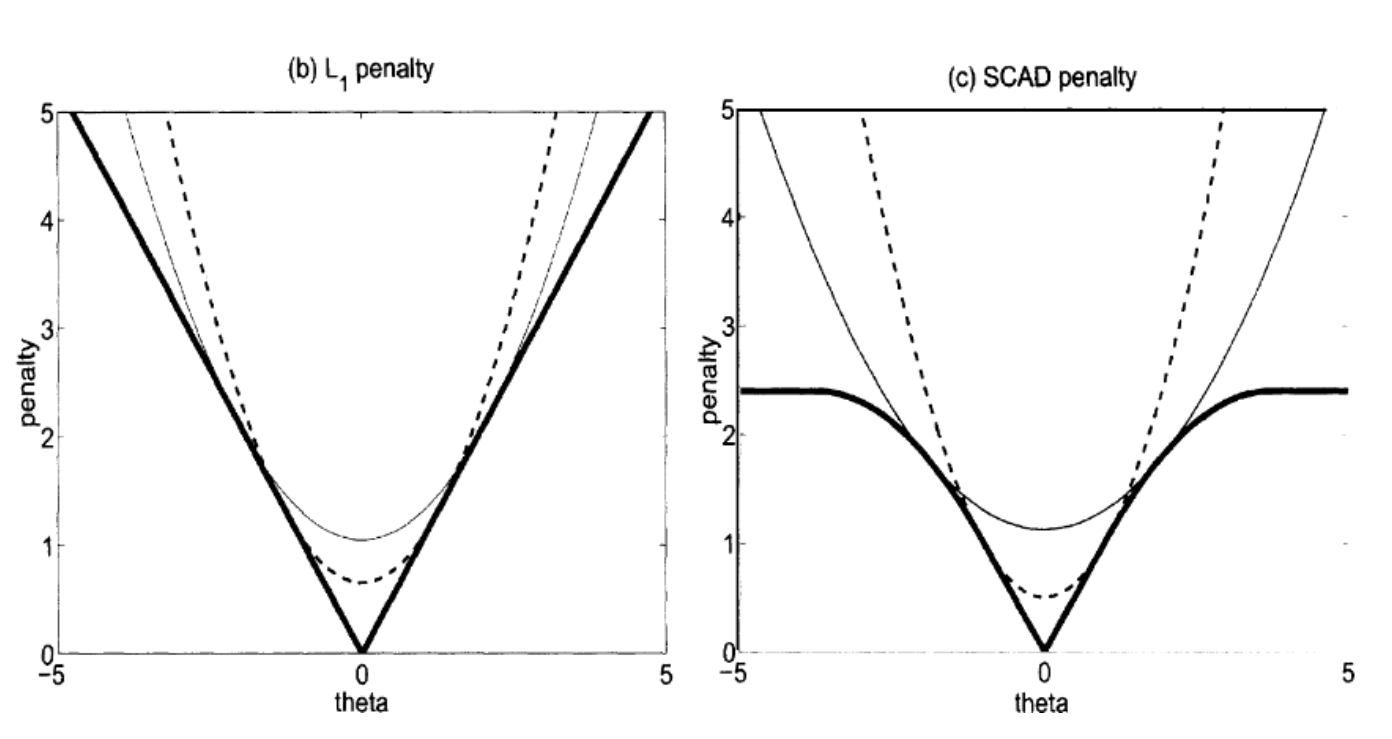
\includegraphics[width=0.4\textwidth]{SCAD}
			\end{center}
			\footnotehint{   
				Fan和Li (2001)  提出 SCAD(smoothly clipped absolute deviation) 罚项: 
				$$
				p_\lambda(|\theta|)=\lambda\left\{I(|\theta| \leq \lambda)+\frac{(a \lambda-|\theta|)_{+}}{(a-1) \lambda} I(|\theta|>\lambda)\right\}
				$$
				其中 $a>2$ 是某个既定的常数  $a=3.7$ 时,Bayes风险较低且模型通常表现的较好。 
				SCAD 惩罚项 具有无偏性、稀疏性和连续性。
			}
		\end{itemize}}
		
	\end{frame}
	
	%-------------------------------------------------------
	\begin{frame}
		\frametitle{拟凸优化问题\zixue}
		\textbf{ $f_{0}$}水平集的凸表示\\
		如果$f_{0}$是拟凸函数, 存在一系列函数 $\phi_{t}$:
		\begin{itemize}[<+->]
			\item 固定 $t$,$\phi_{t}(x)$ 在 $x$上 是凸函数
			\item $f_{0}$的 $t$-水平集 是 $\phi_{t}$的 0-水平集, $i.e.$,
			\begin{equation}
				f_{0}(x) \leq t \quad \Longleftrightarrow \quad \phi_{t}(x) \leq 0
			\end{equation}
		\end{itemize}
	\end{frame}
	
	\begin{frame}
		\onslide<3->{
			\highlight{ 例.}
				\begin{equation}
					f_{0}(x)=\frac{p(x)}{q(x)}
				\end{equation}
				$p$ 为凸函数, $q$ 为凹函数, 且 $p(x) \geq 0, q(x)>0$ 在 $\textbf{dom}\ f_{0}$
				可以得到 $\phi_{t}(x)=p(x)-t q(x)$
				\begin{itemize}[<+->]
					\item  $\forall t \geq 0, \phi_{t}$ 在$x$处为凸函数 
					\item $p(x) / q(x) \leq t$ 当且仅当 $\phi_{t}(x) \leq 0$
				\end{itemize}
		}
  	\end{frame}
	%-------------------------------------------------------
	\begin{frame}
		\frametitle{拟凸优化问题\zixue}
		\textbf{基于凸可行性问题的拟凸优化}
		\begin{equation}
			\phi_{t}(x) \leq 0, \quad f_{i}(x) \leq 0, \quad i=1, \ldots, m, \quad A x=b
		\end{equation}
		\begin{itemize}[<+->]
			\item 对于固定的 $t,$ 是$x$中的一个凸可行问题
			\item 如果可行,我们可以得出结论 $t \geq p^{\star} ;$ 如果不可行, $t \leq p^{\star}$
		\end{itemize}
		\onslide<3->{
			\hrule
			
			%$Bisection\ method\ for\ quasiconvex\ optimization$\\
			拟凸优化的 bisection 优化算法
			\textbf{给定} $l \leq p^{\star}, u \geq p^{\star},$ 容忍度 $\epsilon>0$\\
			\textbf{循环}\\
			\quad1. $t:=(l+u) / 2$.\\
			\quad2. 解决凸可行性问题(33).\\
			\quad3. \textbf{如果式} (33) 是可行的, $u:=t ; \quad$ \textbf{否则} $l:=t$ \\
			\textbf{直到} $u-l \leq \epsilon$\\
			
			\hrule
			\bigskip 
			
			需要 $\left\lceil\log _{2}((u-l) / \epsilon)\right\rceil$ 迭代 (其中 $u, l$ 是初始值)
		}
	\end{frame}
	\fi
	%==============================================================
	\subsection{线性规划}
	\begin{frame}
		\frametitle{线性规划(LP)}
		\begin{equation}
			\begin{array}{ll}
				\text { minimize } & c^{T} x+d \\
				\text { subject to } & G x \preceq h \\
				& A x=b
			\end{array}
		\end{equation}
		\begin{itemize}[<+->]
			\item 目标函数和约束条件都是仿射函数的凸问题
			\item 可行集是多面体
		\end{itemize}
		\onslide<3->{
			\begin{figure}
				\centering
				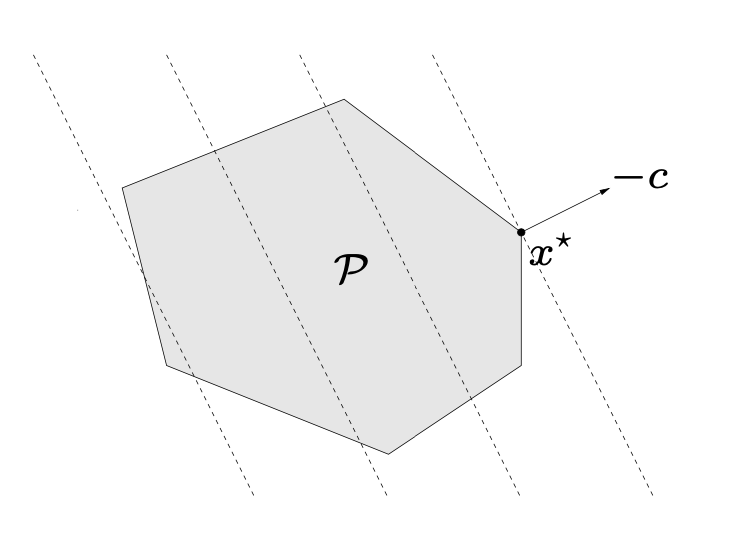
\includegraphics[height=5cm,width=7cm]{Ch4-Linear-program}	
			\end{figure}
		}
	\end{frame}
	%-------------------------------------------------------
	\begin{frame}
		\frametitle{示例}
		\textbf{1.饮食问题:} 选择$n$ 种食物的数量  $x_{1}, \ldots, x_{n}$
		\begin{itemize}
			\item 一个单位的食物 $j$ 花费 $c_{j}$, 包含的营养$i$的数量为 $a_{i j}$ 
			\item 健康饮食需要的营养 $i$ 在数量上至少为 $b_{i}$
		\end{itemize}
		为了找到最便宜的健康饮食方案,
		\begin{equation}
			\begin{array}{ll}
				\text{ minimize } & c^{T} x \\
				\text { subject to } & A x \succeq b, \quad x \succeq 0
			\end{array}
		\end{equation}
		\\
		\onslide<2->{
			\textbf{2. 分段线性最小化问题}
			\begin{equation}
				\text { minimize } \max _{i=1, \ldots, m}\left(a_{i}^{T} x+b_{i}\right)
			\end{equation}
			等价于一个 LP问题
			\begin{equation}
				\begin{array}{ll}
					\text { minimize } & t \\
					\text { subject to } & a_{i}^{T} x+b_{i} \leq t, \quad i=1, \ldots, m
				\end{array}
			\end{equation}
		}
	\end{frame}
	%-------------------------------------------------------
	\begin{frame}
		\frametitle{示例}
		\begin{columns}
			\column{0.5\textwidth}
			\textbf{3. 多面体的切比雪夫中心}\\
			\begin{equation}
				\mathcal{P}=\left\{x \mid a_{i}^{T} x \leq b_{i}, i=1, \ldots, m\right\}
			\end{equation}
			的切比雪夫中心是最大内切球的中心
			\begin{equation}
				\mathcal{B}=\left\{x_{c}+u \mid\|u\|_{2} \leq r\right\}
			\end{equation}
			\onslide<2->{
				\column{0.5\textwidth}
				\begin{figure}
					\centering
					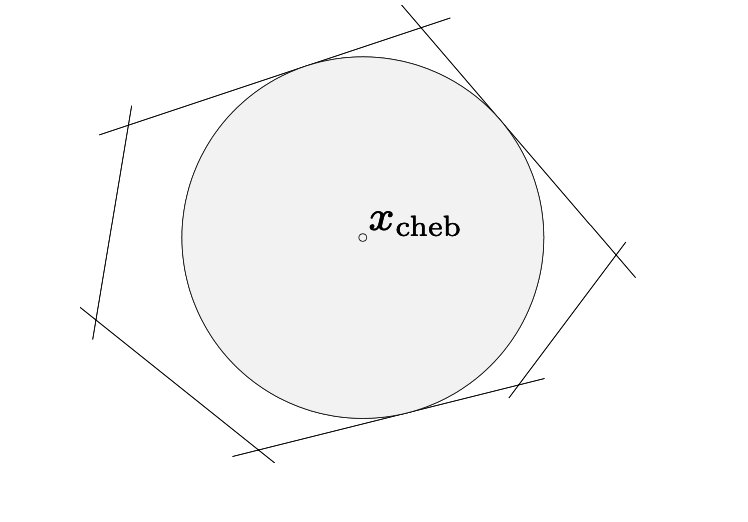
\includegraphics[ width=  0.89\textwidth]{Ch4-Chebyshev-center-of-a-polyhedron}
				\end{figure}
			}
		\end{columns}
		\onslide<3->{
			\begin{itemize}[<+->]
				\item $a_{i}^{T} x \leq b_{i}$  $\forall x \in \mathcal{B}$ 当且仅当
				\begin{equation}
					\sup \left\{a_{i}^{T}\left(x_{c}+u\right) \mid\|u\|_{2} \leq r\right\}=a_{i}^{T} x_{c}+r\left\|a_{i}\right\|_{2} \leq b_{i}
				\end{equation}
				
				\item 因此, $x_{c}, r$ 可以通过求解LP问题来确定
				\begin{equation}
					\begin{array}{ll}
						\text{ maximize } & $r$ \\
						\text { subject to } & a_{i}^{T} x_{c}+r\left\|a_{i}\right\|_{2} \leq b_{i}, \quad i=1, \ldots, m
					\end{array}
				\end{equation}
			\end{itemize}
		}
	\end{frame}
	
	
	\begin{frame}
		\frametitle{例.基于线性规划求解该多面体的切比雪夫中心}
		
		考虑下面的线性不等式组定义的多面体 $\mathcal{P}$ :
		$$
		\left[\begin{array}{cc}
			1 & 1 \\
			1 & -1 \\
			-1 & 0
		\end{array}\right] \cdot\left[\begin{array}{l}
			y \\
			x
		\end{array}\right] \preccurlyeq\left[\begin{array}{l}
			1 \\
			1 \\
			0
		\end{array}\right]
		$$
	 运行代码,基于线性规划求解该多面体的切比雪夫中心
		\end{frame}
		
		\begin{frame}
		\frametitle{基于线性规划求解该多面体的切比雪夫中心(运行代码)}
		\small{
		1 from scipy import optimize\\
		2 import numpy as np\\
		3 from matplotlib import pyplot as plt\\
		4 c = np.array([1,0,0])\\
		5 A = np.array([[np.sqrt(2),1,1],[np.sqrt(2),1,1],[1,-1,0]])\\
		6 b = np.array([1,1,0])\\
		7 res = optimize.linprog(-c,A,b)\\
		8 res.x\\
		9 plt.plot([-1,0],[0,1],'b')\\
		10 plt.plot([0,1],[1,0],'b')\\
		11 plt.plot([-1,1],[0,0],'b')\\
		12 r,x,y = res.x[0],res.x[2],res.x[1]\\
		13 theta = np.arange(0,2*np.pi,0.01)\\
		14plt.plot(x+r*np.cos(theta),y+r*np.sin(theta),'r')\\
		15 plt.plot(x,y,'k.')\\
		16 plt.axis('equal')\\
		}
	   	\end{frame}
	
     \begin{frame}
	\begin{figure}
		\centering
		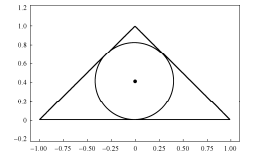
\includegraphics[ width=  0.7\textwidth]{Ch4-Chebyshev-center}
	\end{figure}
	多面体P及求得的切比雪夫中心,如图所示。
	\end{frame}
	%-------------------------------------------------------
	\iffalse
	\begin{frame}
		\frametitle{例. 线性分式规划 (Ex.)}
		\begin{equation}
			\begin{array}{ll}
				\text{ minimize } & f_{0}(x) \\
				\text { subject to } & G x \preceq h \\
				& A x=b
			\end{array}
		\end{equation}
		\onslide<2->{
			\textbf{线性分式规划}
			\begin{equation}
				f_{0}(x)=\frac{c^{T} x+d}{e^{T} x+f}, \quad \textbf{dom}\ f_{0}(x)=\left\{x \mid e^{T} x+f>0\right\}
			\end{equation}
		}
		\onslide<3->{
			\begin{itemize}[<+->]
				\item \blue{一个拟凸优化问题;} 可以通过二等分来解决
				\item 也等价于LP问题: \dred{$x= y/z$, $e^{T} y+f z=1 $, $z \geq 0$} %(variables $y,z$)
			\end{itemize}
			\begin{equation}
				\begin{array}{ll}
					\text{ minimize } & c^{T} y+d z \\
					\text { subject to } & G y \preceq h z \\
					& A y=b z \\
					& e^{T} y+f z=1 \\
					& z \geq 0
				\end{array}
			\end{equation}
		}
	\end{frame}
	%-------------------------------------------------------
	\begin{frame}
		\frametitle{例. 线性分式规划(Ex.)}
		\textbf{广义线性分式规划}
		\begin{equation}
			f_{0}(x)=\max _{i=1, \ldots, r} \frac{c_{i}^{T} x+d_{i}}{e_{i}^{T} x+f_{i}}, \quad \textbf{dom}\ f_{0}(x)=\left\{x \mid e_{i}^{T} x+f_{i}>0, i=1, \ldots, r\right\}
		\end{equation}
		\onslide<2->{
			一个拟凸优化问题;可以通过二等分来解决\\
		}
		
	\end{frame}
	
	
	\begin{frame}
		
			\highlight{ 例.}(经济增长的 Von Neumann 模型)
		
			\begin{equation}
				\begin{array}{ll}
					\text { maximize (over} \left.x, x^{+}\right) & \min _{i=1, \ldots, n} x_{i}^{+} / x_{i} \\
					\text { subject to } & x^{+} \succeq 0, \quad B x^{+} \preceq A x
				\end{array}
			\end{equation}
			\begin{itemize}[<+->]
				\item $x, x^{+} \in \mathbb{R}^{n}$: 
				当前期/下一期的$n$ 个经济部门的活跃度(activity level)
				%s of $n$ sectors, in current and next period
				
				\item $(A x)_{i},\left(B x^{+}\right)_{i}:$ 
				%produced, resp. consumed, amounts of good $i$
				商品 $i$ 的生产量 / 消费量
				
				\item $x_{i}^{+} / x_{i}:$ 部门$i$ 的增长率 
				%growth rate of sector $i$
				
				\item 目标: 优化各部门活跃度 最大化 最低增长率  
				%allocate activity to maximize growth rate of slowest growing sector
			\end{itemize}
		\end{frame}
	\fi
	%==============================================================
	\subsection{二次规划}
	\begin{frame}
		\frametitle{二次规划 (QP)}
		\begin{equation}
			\begin{array}{ll}
				\text { minimize } & (1 / 2) x^{T} P x+q^{T} x+r \\
				\text { subject to } & G x \preceq h \\
				& A x=b
			\end{array}
		\end{equation}
		\begin{itemize}[<+->]
			\item $P \in \mathbf{S}_{+}^{n}$, 所以目标是凸二次函数
			\item 最小化多面体上的凸二次函数
		\end{itemize}
		\onslide<3->{
			\begin{figure}
				\centering
				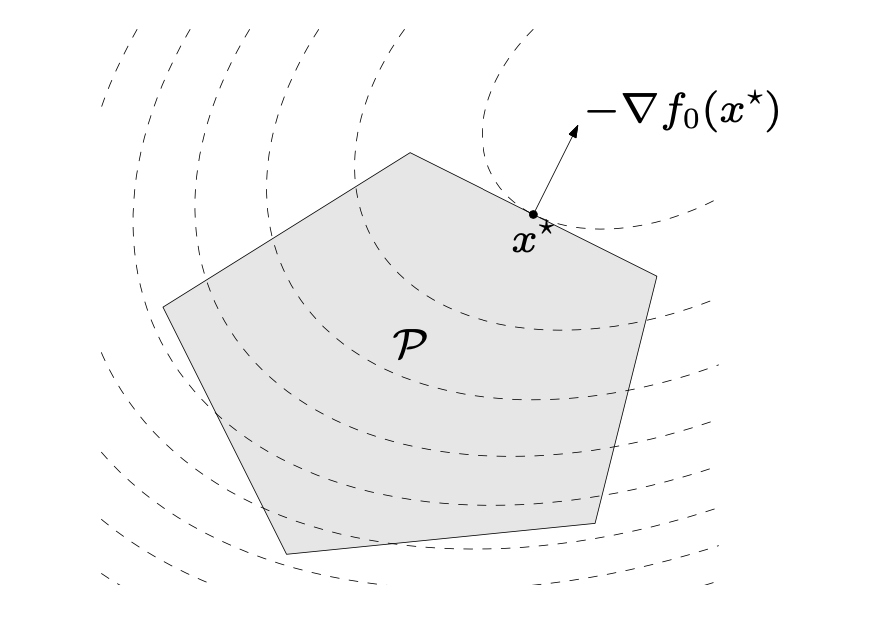
\includegraphics[height=5cm,width=6cm]{Ch4-Quadratic-program}
			\end{figure}
		}
	\end{frame}
	%-------------------------------------------------------
	\begin{frame}
		\frametitle{示例}
		\textbf{1.最小二乘回归}
		\begin{equation}
			\text { minimize } \quad\frac{1}{2}\|A x-b\|_{2}^{2}
		\end{equation}
		\begin{itemize}
			\item 解析解 $x^{\star}=A^{\dagger} b\left(A^{\dagger}\right.$ 是$A$的伪逆 $)$
			\item 可以添加线性约束, $e . g ., l \preceq x \preceq u$
		\end{itemize}
		
		\onslide<2->{
			\textbf{2.具有随机成本的线性规划}
			\begin{equation}
				\begin{array}{ll}
					\text { minimize } & \bar{c}^{T} x+\gamma x^{T} \Sigma x=\mathbf{E} c^{T} x+\gamma \textbf{var}\left(c^{T} x\right) \\
					\text { subject to } & G x \preceq h, \quad A x=b
				\end{array}
			\end{equation}
			\begin{itemize}[<+->]
				\item $c$ 是具有均值 $\bar{c}$ 和协方差$\Sigma$的随机向量 
				\item 因此, $c^{T} x$ 是具有平均值 $\bar{c}^{T} x$ 和方差$x^{T} \Sigma x$的随机变量
				\item $\gamma>0$ 是风险规避参数;控制预期成本和差异(风险)之间的权衡
			\end{itemize}
		}
	\end{frame}
	
	\begin{frame}
		
			\onslide<2->{
			\textbf{3.多面体之间的距离}
		\begin{itemize}
			\item 
			多面体 $\mathcal{P}_1=\left\{\boldsymbol{x} \mid \boldsymbol{A}_1 \boldsymbol{x} \preceq \boldsymbol{b}_1\right\}$ 和 $\mathcal{P}_2=\left\{\boldsymbol{x} \mid \boldsymbol{A}_2 \boldsymbol{x} \preceq \boldsymbol{b}_2\right\}$ 在 $\mathbf{R}^n$ 上的欧氏距离定义为
			$$
			\operatorname{dist}\left(\mathcal{P}_1, \mathcal{P}_2\right)=\inf \left\{\left\|\boldsymbol{x}_1-\boldsymbol{x}_2\right\|_2 \mid \boldsymbol{x}_1 \in \mathcal{P}_1, \boldsymbol{x}_2 \in \mathcal{P}_2\right\}
			$$
			\item 如果多面体相交,则距离为零。
			\item  求解下面的二次规划 $\rightarrow$  $\mathcal{P}_1$ 和 $\mathcal{P}_2$ 之间的距离 
			$$
			\begin{array}{ll}
				\text { minimize }_{ \boldsymbol{x}_1, \boldsymbol{x}_2 \in \mathbf{R}^n} & \left\|\boldsymbol{x}_1-\boldsymbol{x}_2\right\|_2^2 \\
				\text { subject to } & \boldsymbol{A}_1 \boldsymbol{x}_1 \preceq \boldsymbol{b}_1, \boldsymbol{A}_2 \boldsymbol{x}_2 \preceq \boldsymbol{b}_2
			\end{array}
			$$
			
			\item 当且仅当 多面体相交时,最优 值为零,  否则最优解 $\boldsymbol{x}_1$ 和 $\boldsymbol{x}_2$ 分 别是 $\mathcal{P}_1$ 和 $\mathcal{P}_2$ 中 最接近的点
			
			%当且仅当其中一个多面体为空时,这个问题是不可行的。当且仅当多面体相交时,最优 值为零, 在这种情况下, 最优解 $\boldsymbol{x}_1$ 和 $\boldsymbol{x}_2$ 相等 (并且是 $\mathcal{P}_1$ 和 $\mathcal{P}_2$ 的交点), 否则最优解 $\boldsymbol{x}_1$ 和 $\boldsymbol{x}_2$ 分 别是 $\mathcal{P}_1$ 和 $\mathcal{P}_2$ 中彼此最接近的点。
			
			
		\end{itemize}
	}
	\end{frame}
	
	\begin{frame}
		
		\frametitle{  例.二次规划求多面体间的距离}
		考虑多面体 $\mathcal{P}_1$
		$$
		\left[\begin{array}{cc}
			1 & 1 \\
			1 & -1 \\
			-1 & 0
		\end{array}\right] \cdot\left[\begin{array}{l}
			y \\
			x
		\end{array}\right] \preccurlyeq\left[\begin{array}{l}
			1 \\
			1 \\
			0
		\end{array}\right]
		$$
		和多面体 $\mathcal{P}_2$
		$$
		\left[\begin{array}{cc}
			0 & -1 \\
			-1 & 1 \\
			1 & 1
		\end{array}\right] \cdot\left[\begin{array}{c}
			y \\
			x
		\end{array}\right] \preccurlyeq\left[\begin{array}{c}
			-2 \\
			2 \\
			4
		\end{array}\right]
		$$
		之间的距离。
		\end{frame}
		
		\begin{frame}
  	学习实例代码 3.4.1,  基于二次规划求解上述两个多面体之间距离。\\
  	代码输出求得的最优解为:[5.30e−04,1.00e+00,5.78e−04,2.00e+00],表示两个多面体相距最近的两个点近似为(1,0)和(2,0)。
		\begin{figure}
			\centering
			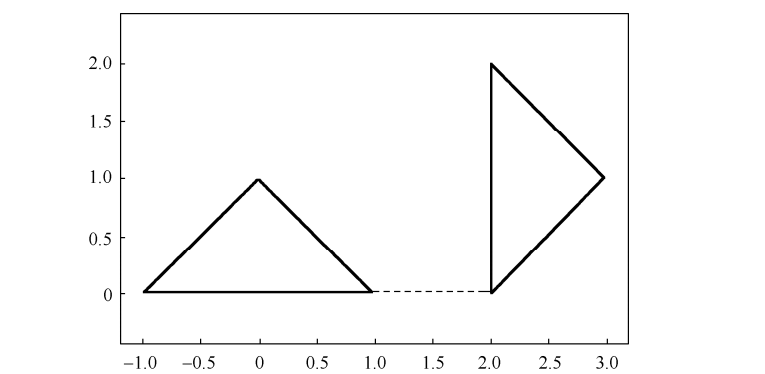
\includegraphics[height=5cm,width=8cm]{Ch4-the-distance-between-polyhedra}
		\end{figure}
		
		如图展示了这两个多面体及其最相距最近的两个点。 
		\end{frame}
		
		
		
		

	%-------------------------------------------------------
	\begin{frame}
		\frametitle{二次约束二次规划(QCQP)}
		
		
		\begin{equation}
			\begin{array}{ll}
				\text { minimize } & (1 / 2) x^{T} P_{0} x+q_{0}^{T} x+r_{0} \\
				\text { subject to } & (1 / 2) x^{T} P_{i} x+q_{i}^{T} x+r_{i} \leq 0, \quad i=1, \ldots, m \\
				& A x=b
			\end{array}
		\end{equation}\\
		\begin{itemize}
			\item $P_{i} \in \mathbf{S}_{+}^{n} ;$ 目标函数和约束函数是凸二次函数 
			\item 如果 $P_{1}, \ldots, P_{m} \in \mathbf{S}_{++}^{n},$ 可行域是$m$个椭球和仿射集$Ax=b$的交集
		\end{itemize}
	\end{frame}
	
	\begin{frame}
		\frametitle{例. QCQP}
		
		\begin{center}
			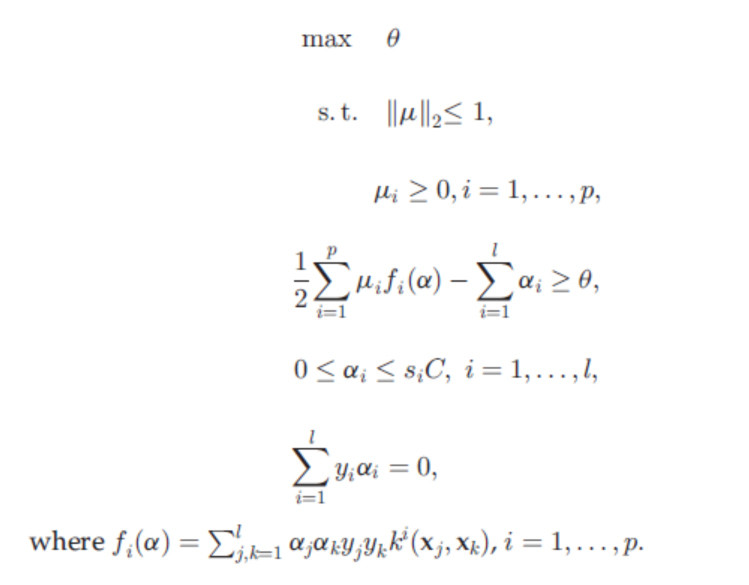
\includegraphics[width = 0.8\textwidth]{QCQP}
		\end{center}
		
		\begin{tiny}
			Ling Jian, Zhonghang Xia, Xinnan Niu, Xijun Liang, Parimal Samir, Andrew J. Link:L2基于多核模糊支持向量机的多肽识别数据融合. IEEE ACM Trans. Comput. Biol. Bioinform. 13(4): 804-809 (2016)
		\end{tiny}
		
		
	\end{frame}
	%-------------------------------------------------------
	\begin{frame}
		\frametitle{二阶锥规划}
		\begin{equation}
			\begin{array}{ll}
				\text{ minimize } & f^{T} x \\
				\text { subject to } & \left\|A_{i} x+b_{i}\right\|_{2} \leq c_{i}^{T} x+d_{i}, \quad i=1, \ldots, m \\
				& F x=g \\
			\end{array}
		\end{equation}
		($A_{i} \in \mathbb{R}^{n_{i} \times n},F \in \mathbb{R}^{p \times n}$)\\
		\begin{itemize}[<+->]
			\item 不等式称为二阶锥(SOC)约束:
			\begin{equation}
				\left(A_{i} x+b_{i}, c_{i}^{T} x+d_{i}\right) \in \mathbb{R}^{n_{i}+1}\text { 上的二阶锥}
			\end{equation}
			
			\hint{
				$\mathbb{R}^{n+1}$上的二阶锥:
				$\{(x,t)\in \mathbb{R}^{n +1} | \|x\|_2 \leq t\}$
			}
			\item 当 $n_{i}=0时,$ 简化成LP问题; 如果 $c_{i}=0,$ 变为一个QCQP问题
			\item 比QCQP和LP更普遍
		\end{itemize}
	\end{frame}
	%-------------------------------------------------------
	\begin{frame}
		\frametitle{例. 鲁棒线性规划}
		优化问题中的参数通常是不确定的, $e.g.$, 在 LP问题中
		\begin{equation}
			\begin{array}{ll}
				\text { minimize } & c^{T} x \\
				\text { subject to } & a_{i}^{T} x \leq b_{i}, \quad i=1, \ldots, m
			\end{array}
		\end{equation}
		在$c$, $a_i$, $b_i$中可能存在不确定性\\
		\onslide<2->{
			处理不确定性的两种常见方法(为了简单起见,以$a_i$为例)
		}
		\onslide<3->{
			\begin{itemize}[<+->]
				\item 确定性模型: 约束必须适用于所有 $a_{i} \in \mathcal{E}_{i}$
				\begin{equation}
					\begin{aligned}
						&\text { minimize } \quad c^{T} x\\
						&\text { subject to } \quad a_{i}^{T} x \leq b_{i} \quad \forall a_{i} \in \mathcal{E}_{i}, \quad i=1, \ldots, m
					\end{aligned}
				\end{equation}
				
				\item 随机模型: $a_{i}$ 为随机变量;约束为概率 约束
				\begin{equation}
					\begin{array}{ll}
						\text{ minimize } & c^{T} x \\
						\text { subject to } & \textbf {prob}\left(a_{i}^{T} x \leq b_{i}\right) \geq \eta, \quad i=1, \ldots, m
					\end{array}
				\end{equation}
			\end{itemize}
		}
	\end{frame}
	%-------------------------------------------------------
	\begin{frame}
		\frametitle{例. 鲁棒线性规划}
		\textbf{确定性方法 $\leftarrow$ SOCP(二阶锥规划)\zixue}
		\begin{itemize}[<+->]
			\item 选择椭球 $\mathcal{E}_{i}$ :
			\begin{equation}
				\mathcal{E}_{i}=\left\{\bar{a}_{i}+P_{i} u \mid\|u\|_{2} \leq 1\right\} \quad\left(\bar{a}_{i} \in \mathbb{R}^{n}, \quad P_{i} \in \mathbb{R}^{n \times n}\right)
			\end{equation}
			球心是 $\bar{a}_{i},$ 由奇异值/向量$P_{i}$确定半轴
			\item 鲁棒线性规划问题
			\begin{equation}
				\begin{array}{ll}
					\text { minimize } & c^{T} x \\
					\text { subject to } & a_{i}^{T} x \leq b_{i} \quad \forall a_{i} \in \mathcal{E}_{i}, \quad i=1, \ldots, m
				\end{array}
			\end{equation}
			等价于 SOCP(二阶锥规划)
			\begin{equation}
				\begin{array}{ll}
					\text { minimize } & c^{T} x \\
					\text { subject to } & \bar{a}_{i}^{T} x+\left\|P_{i}^{T} x\right\|_{2} \leq b_{i}, \quad i=1, \ldots, m
				\end{array}
			\end{equation}
			由于 $\left.\sup _{\|u\|_{2} \leq 1}\left(\bar{a}_{i}+P_{i} u\right)^{T} x=\bar{a}_{i}^{T} x+\left\|P_{i}^{T} x\right\|_{2}\right)$
		\end{itemize}
	\end{frame}
	%-------------------------------------------------------
	\begin{frame}
		\frametitle{基于 SOCP(二阶锥规划) 的 随机方法 }
		\begin{itemize}[<+->]
			\item 假定 $a_{i}$ 为高斯分布,均值为 $\bar{a}_{i},$ 方差为 $\Sigma_{i}\left(a_{i} \sim \mathcal{N}\left(\bar{a}_{i}, \Sigma_{i}\right)\right)$
			\item $a_{i}^{T} x$ 是一个高斯$r . v .$ ,均值为 $\bar{a}_{i}^{T} x,$ 方差为 $x^{T} \Sigma_{i} x ;$ 
			\begin{equation}
				\textbf{prob}\left(a_{i}^{T} x \leq b_{i}\right)=\Phi\left(\frac{b_{i}-\bar{a}_{i}^{T} x}{\left\|\Sigma_{i}^{1 / 2} x\right\|_{2}}\right)
			\end{equation}
			其中 $\Phi(x)=(1 / \sqrt{2 \pi}) \int_{-\infty}^{x} e^{-t^{2} / 2} d t$ 是 $\mathcal{N}(0,1)$的分布函数\\
			\item 鲁棒线性规划
			\begin{equation}
				\begin{array}{ll}
					\text{ minimize } & c^{T} x \\
					\text { subject to } & \textbf {prob}\left(a_{i}^{T} x \leq b_{i}\right) \geq \eta, \quad i=1, \ldots, m
				\end{array}
			\end{equation}
			$\eta \geq 1 / 2,$ 等价于 SOCP问题
			\begin{equation}
				\begin{array}{ll}
					\text{ minimize } & c^{T} x \\
					\text { subject to } & \bar{a}_{i}^{T} x+\Phi^{-1}(\eta)\left\|\Sigma_{i}^{1 / 2} x\right\|_{2} \leq b_{i}, \quad i=1, \ldots, m
				\end{array}
			\end{equation}
		\end{itemize}
	\end{frame}
	
	
	\begin{frame}
		\frametitle{  例. 二阶雉规划问题}
		$$
		\begin{aligned}
			\text { minimize } & -2 x_1+x_2+5 x_3 \\
			\text { subject to } & \left\|\left[\begin{array}{c}
				-13 x_1+3 x_2+5 x_3-3 \\
				-12 x_1+12 x_2-6 x_3-2
			\end{array}\right]\right\|_2 \leqslant-12 x_1-6 x_2+5 x_3-12 \\
			& \left\|\left[ \begin{array}{c}
				-3 x_1+6 x_2+2 x_3 \\
				x_1+9 x_2+2 x_3+3 \\
				-x_1-19 x_2+3 x_3-42
			\end{array}\right] \right\|_2 \leqslant-3 x_1+6 x_2-10 x_3+27
		\end{aligned}
		$$
		
		学习实例代码 3.4.2,
		调用 Cvxopt 包求解上述问题,  所求得的最优解为 $[-5.01 \mathrm{e}+00$, $-5.77 \mathrm{e}+00,-8.52 \mathrm{e}+00]$  
	\end{frame}
	
	%===============================================================
	\subsection{几何规划}
	\begin{frame}
		\frametitle{几何规划}
		\textbf{单项式函数}
		\begin{equation}
			f(x)=c x_{1}^{a_{1}} x_{2}^{a_{2}} \cdots x_{n}^{a_{n}}, \quad \textbf { dom } f=\mathbb{R}_{++}^{n}
		\end{equation}
		$c>0$; \dred{ $a_{i}$ 可以为任意实数}\\
		\onslide<2->{
			\textbf{多项式函数:} 单项式求和
			\begin{equation}
				f(x)=\sum_{k=1}^{K} c_{k} x_{1}^{a_{1 k}} x_{2}^{a_{2 k}} \cdots x_{n}^{a_{n k}}, \quad \textbf { dom } f=\mathbb{R}_{++}^{n}
			\end{equation}\\
		}
		\onslide<3->{
			
			\textbf{几何规划 (GP)}
			\begin{equation}
				\begin{array}{ll}
					\text{ minimize } & f_{0}(x) \\
					\text { subject to } & f_{i}(x) \leq 1, \quad i=1, \ldots, m \\
					& h_{i}(x)=1, \quad i=1, \ldots, p
				\end{array}
			\end{equation}
			$f_{i}$ 为多项式, $h_{i}$ 为单项式
		}
	\end{frame}
	%-------------------------------------------------------
	\begin{frame}
		\frametitle{凸形几何规划}
		将变量更改为\dred{$y_{i}=\log x_{i},$} 并取目标和约束条件的对数\\
		\begin{itemize}[<+->]
			\item 单项式 $f(x)=c x_{1}^{a_{1}} \cdots x_{n}^{a_{n}}$ 变为
			\begin{equation}
				\log f\left(e^{y_{1}}, \ldots, e^{y_{n}}\right)=a^{T} y+b \quad(b=\log c)
			\end{equation}
			
			\item 多项式 $f(x)=\sum_{k=1}^{K} c_{k} x_{1}^{a_{1 k}} x_{2}^{a_{2 k}} \cdots x_{n}^{a_{n k}}$ 变为
			\begin{equation}
				\log f\left(e^{y_{1}}, \ldots, e^{y_{n}}\right)=\log \left(\sum_{k=1}^{K} e^{a_{k}^{T} y+b_{k}}\right) \quad\left(b_{k}=\log c_{k}\right)
			\end{equation}
			
			\item 几何规划转变为凸问题
			\begin{equation}
				\begin{array}{ll}
					\text { minimize } & \log \left(\sum_{k=1}^{K} \exp \left(a_{0 k}^{T} y+b_{0 k}\right)\right) \\
					\text { subject to } & \log \left(\sum_{k=1}^{K} \exp \left(a_{i k}^{T} y+b_{i k}\right)\right) \leq 0, \quad i=1, \ldots, m \\
					& G y+d=0
				\end{array}
			\end{equation}
		\end{itemize}
	\end{frame}
	%-------------------------------------------------------
	\begin{frame}
		\frametitle{悬臂梁设计}
		\begin{figure}
			\centering
			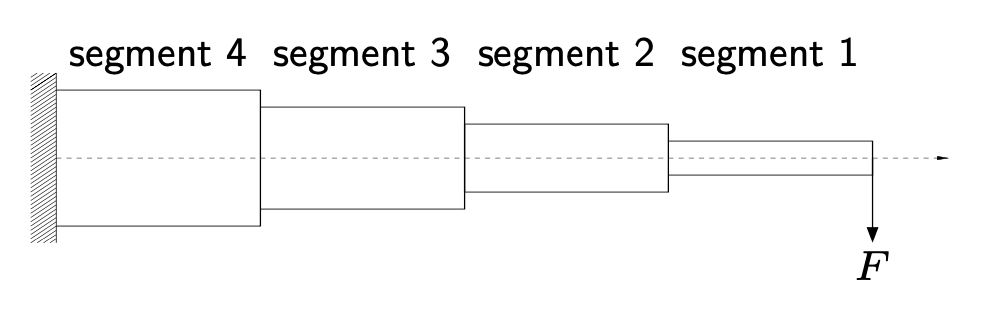
\includegraphics[height=3cm,width=8cm]{Ch4-Design-of-cantilever-beam}	
		\end{figure}
		\begin{itemize}%[<+->]
			\item 具有单位长度的线段$N$ ,大小 $w_i \times h_i$为矩形截面
			\item 给定右端施加的垂直力$F$
		\end{itemize}
		\onslide<3->{
			\textbf{设计问题}
			\begin{equation}
				\begin{array}{ll}
					\text{ minimize } & \text{总重量}\\
					\text{ subject to } & 
					w_{i}, h_{i}\text{ 上下界 }\\ 
					& \text{纵横比 (aspect ratio)}  h_{i} / w_{i} \text{的上下界}\\ 
					&\text{每段应力的上下界 }
					\\
					&  
					\text{每段末尾 的垂直偏转(vertical deflection) 力的上界 }\\
				\end{array}
			\end{equation}
			\quad \text{变量}: $w_i, h_i$\text{ for }$i = 1,\cdots,N$
		}
	\end{frame}
	%-------------------------------------------------------
	\begin{frame}
		\frametitle{悬臂梁设计}
		\textbf{目标函数和约束条件}\\
		
		\begin{itemize}[<+->]
			\item 总重量$w_{1} h_{1}+\cdots+w_{N} h_{N}$ 是多项式
			
			\item 纵横比 $h_{i} / w_{i}$ 和反纵横比$w_{i} / h_{i}$ 是单项式
			
			\item 线段$i$ 中的最大应力由一个单项式给出$6 i F /\left(w_{i} h_{i}^{2}\right)$ 
			
			\item 线段 $i$右端中心轴的垂直偏转$y_{i}$和斜率$v_{i}$递归定义为
			\begin{equation}
				\begin{array}{l}
					v_{i}=12(i-1 / 2) \frac{F}{E w_{i} h_{i}^{3}}+v_{i+1} \\
					y_{i}=6(i-1 / 3) \frac{F}{E w_{i} h_{i}^{3}}+v_{i+1}+y_{i+1}
				\end{array}
			\end{equation}
			$i=N, N-1, \ldots, 1,$  $v_{N+1}=y_{N+1}=0(E$ 是杨氏模量)\\
			$v_{i}$ 和 $y_{i}$ 是$w, h$的多项式函数  
		\end{itemize}
	\end{frame}
	%-------------------------------------------------------
	\begin{frame}
		\frametitle{悬臂梁设计}
		\textbf{构造一个 GP问题}
		\begin{equation}
			\begin{array}{ll}
				\text { minimize } & w_{1} h_{1}+\cdots+w_{N} h_{N} \\
				\text { subject to } & w_{\max }^{-1} w_{i} \leq 1, \quad w_{\min } w_{i}^{-1} \leq 1, \quad i=1, \ldots, N \\
				& h_{\max }^{-1} h_{i} \leq 1, \quad h_{\min } h_{i}^{-1} \leq 1, \quad i=1, \ldots, N \\
				& S_{\max }^{-1} w_{i}^{-1} h_{i} \leq 1, \quad S_{\min } w_{i} h_{i}^{-1} \leq 1, \quad i=1, \ldots, N \\
				& 6 i F \sigma_{\max }^{-1} w_{i}^{-1} h_{i}^{-2} \leq 1, \quad i=1, \ldots, N \\
				& y_{\max }^{-1} y_{1} \leq 1
			\end{array}
		\end{equation}\\
		
		\onslide<2->{
			注意
			\begin{itemize}[<+->]
				\item   $w_{\min } \leq w_{i} \leq w_{\max }$, $h_{\min } \leq h_{i} \leq h_{\max }$ $\rightarrow$
				\begin{equation}
					w_{\min } / w_{i} \leq 1, \quad w_{i} / w_{\max } \leq 1, \quad h_{\min } / h_{i} \leq 1, \quad h_{i} / h_{\max } \leq 1
				\end{equation}
				\item   $S_{\min } \leq h_{i} / w_{i} \leq S_{\max }$  $\leftarrow$
				\begin{equation}
					S_{\min } w_{i} / h_{i} \leq 1, \quad h_{i} /\left(w_{i} S_{\max }\right) \leq 1
				\end{equation}
			\end{itemize}
		}
	\end{frame}
	%-------------------------------------------------------
	\begin{frame}
		\frametitle{最小化非负矩阵的谱半径}
		\textbf{erron-Frobenius特征值} $\lambda_{\text{pf}}(A)$
		\begin{itemize}[<+->]
			\item 存在对每个元素都为正的矩阵 $A \in \mathbb{R}^{n \times n}$
			\item 实际的正特征值$A,$ 等于光谱半径 $\max _{i}\left|\lambda_{i}(A)\right|$
			\item 确定 $A^{k}$ 的渐近增长(衰减)率:$ A^{k} \sim \lambda_{\mathrm{pf}}^{k}$ as $k \rightarrow \infty$
			\item \hint{替代性特征: $\lambda_{\mathrm{pf}}(A)=\inf \{\lambda \mid A v \preceq \lambda v$ for some $v \succ 0\}$}
		\end{itemize}
		
		\onslide<5->{
			\textbf{最小化多项式矩阵的谱半径}
			\begin{itemize}[<+->]
				\item 最小化 $\lambda_{\mathrm{pf}}(A(x)),$ 其中 $A(x)_{i j}$ 中元素是$x$的多项式
				\item 等效几何规划: 	
				\begin{equation}
					\begin{array}{ll}
						\text { minimize } & \lambda \\
						\text { subject to } & \sum_{j=1}^{n} A(x)_{i j} v_{j} /\left(\lambda v_{i}\right) \leq 1, \quad i=1, \ldots, n
					\end{array}
				\end{equation}
				变量为 $\lambda, v, x$
			\end{itemize}
		}
	\end{frame}
	%===============================================================
	\subsection{广义不等式约束}
	\begin{frame}
		\frametitle{广义不等式约束}
		\textbf{具有广义不等式约束的凸问题}
		\begin{equation}
			\begin{array}{ll}
				\text{ minimize } & f_{0}(x) \\
				\text { subject to } & f_{i}(x) \preceq_{K_{i}} 0, \quad i=1, \ldots, m \\
				& A x=b
			\end{array}
		\end{equation}
		\begin{itemize}[<+->]
			\item $f_{0}: \mathbb{R}^{n} \rightarrow \mathbb{R}$ 为凸函数; $f_{i}: \mathbb{R}^{n} \rightarrow \mathbb{R}^{k_{i}} K_{i}$ -凸, $K_{i}$: proper cone (正常锥)
			\item 与标准凸问题相同的性质(凸可行集,局部最优解是全局最优的, etc.)
		\end{itemize}
		
		\onslide<3->{
			\textbf{锥形问题:} 具有仿射目标函数和约束条件的特例
			\begin{equation}
				\begin{array}{ll}
					\text{ minimize } & c^{T} x \\
					\text { subject to } & F x+g \preceq_{K} 0 \\
					& A x=b
				\end{array}
			\end{equation}
			将线性规划$\left(K=\mathbb{R}_{+}^{m}\right)$ 推广到非多面体锥
		}
	\end{frame}
	%==============================================================
	\subsection{半定规划Semidefinite program}
	\begin{frame}
		\frametitle{半定规划(SDP)}
		\begin{equation}
			\begin{array}{ll}
				\text { minimize } & c^{T} x \\
				\text { subject to } & x_{1} F_{1}+x_{2} F_{2}+\cdots+x_{n} F_{n}+G \preceq 0 \\
				& A x=b
			\end{array}
		\end{equation}
		其中 $F_{i}, G \in \mathbf{S}^{k}$\\
		\begin{itemize}[<+->]
			\item 不等式约束称为线性矩阵不等式 (LMI)
			\item 包括具有多个LMI约束的问题: 例如,
			\begin{equation}
				x_{1} \hat{F}_{1}+\cdots+x_{n} \hat{F}_{n}+\hat{G} \preceq 0, \quad x_{1} \tilde{F}_{1}+\cdots+x_{n} \tilde{F}_{n}+\tilde{G} \preceq 0
			\end{equation}\\
			等价于 单线矩阵不等式 SLMI
			\begin{equation}
				x_{1}\left[\begin{array}{cc}
					\hat{F}_{1} & 0 \\
					0 & \tilde{F}_{1}
				\end{array}\right]+x_{2}\left[\begin{array}{cc}
					\hat{F}_{2} & 0 \\
					0 & \tilde{F}_{2}
				\end{array}\right]+\cdots+x_{n}\left[\begin{array}{cc}
					\hat{F}_{n} & 0 \\
					0 & \tilde{F}_{n}
				\end{array}\right]+\left[\begin{array}{cc}
					\hat{G} & 0 \\
					0 & \tilde{G}
				\end{array}\right] \preceq 0
			\end{equation}
		\end{itemize}
	\end{frame}
	%-------------------------------------------------------
	\begin{frame}
		\frametitle{特征值最小化}
		\begin{equation}
			\text { minimize } \quad \lambda_{\max }(A(x))
		\end{equation}
		其中 $A(x)=A_{0}+x_{1} A_{1}+\cdots+x_{n} A_{n}$ (给定 $A_{i} \in \mathbf{S}^{k}$ )\\
		
		\onslide<2->{
			等价于 SDP问题
			\begin{equation}
				\begin{array}{ll}
					\text{ minimize } & t \\
					\text { subject to } & A(x) \preceq t I
				\end{array}
			\end{equation}
		}
		\onslide<3->{
			\begin{itemize}[<+->]
				\item 变量 $x \in \mathbb{R}^{n}, t \in \mathbb{R}$
				\item 来自于
				\begin{equation}
					\lambda_{\max }(A) \leq t \quad \Longleftrightarrow \quad A \preceq t I
				\end{equation}
			\end{itemize}
		}
	\end{frame}
	%------------------------------------------------------
	\begin{frame}
		\frametitle{矩阵范数最小化}
		\begin{equation}
			\text{minimize} \quad\|A(x)\|_{2}=\left(\lambda_{\max }\left(A(x)^{T} A(x)\right)\right)^{1 / 2}
		\end{equation}
		其中 $A(x)=A_{0}+x_{1} A_{1}+\cdots+x_{n} A_{n}$ ( $ A_{i} \in \mathbb{R}^{p \times q} $ 给定 )
		\footnotehint{ $\|A\|_2 =  A$的最大奇异值}
		\onslide<2->{
			$\leftrightarrow$ SDP
			\begin{equation}
				\begin{array}{ll}
					\text { minimize } & t\\
					\text { subject to } & \left[\begin{array}{cc}
						t I & A(x) \\
						A(x)^{T} & t I
					\end{array}\right] \succeq 0
				\end{array}
			\end{equation}
		}
		\onslide<3->{
			\begin{itemize}[<+->]
				\item 变量 $x \in \mathbb{R}^{n}, t \in \mathbb{R}$
				\item 约束: 
				\begin{equation}
					\begin{aligned}
						\|A\|_{2} \leq t & \Longleftrightarrow A^{T} A \preceq t^{2} I, \quad t \geq 0 \\
						& \Longleftrightarrow\left[\begin{array}{cc}
							t I & A \\
							A^{T} & t I
						\end{array}\right] \succeq 0
					\end{aligned}
				\end{equation}
			\end{itemize}
		}
	\end{frame}
	
	\begin{frame}
		\frametitle{例.最大割问题的半定规划松弛}
		
		\begin{itemize}
			\item  
			设 $G$ 是一个无向图, 顶点集合为 $\mathbf{N}=1,2, \cdots, n$,边的集合为 $\mathbf{E}$ 
			\item 
			设 $w_{i j}=w_{j i}$ 为边 $(i, j)$ 上 的权值, 其中 $(i, j) \in \mathbf{E}$ 。假设对于所有的 $(i, j) \in \mathbf{E}$, 都有 $w_{i j}>0$ 
			
			\item 最大割问题是指确定顶点 集合 $\mathbf{N}$ 的一个子集 $\mathbf{S}$, 使连接顶点子集 $\mathbf{S}$ 到它的余集 $\overline{\mathbf{S}}$ (其中 $\overline{\mathbf{S}}:=\boldsymbol{N} \backslash \mathbf{S}$ ) 的所有的边权值之 和最大 
			
			\item 
			若 $j \in \mathbf{S}$, 则令 $x_j=-1$, 否则,令 $x_j=1$, 可以将最大割问题描述为如下的整数规划问题: 
			$$
			\begin{array}{ll}
				\text { maximize } & \frac{1}{4} \sum_{i=1}^n \sum_{j=1}^n w_{i j}\left(1-x_i x_j\right) \\
				\text { subject to } & x_j \in\{-1,1\}, j=1,2, \cdots, n
			\end{array}
			$$
			
			
		\end{itemize}
		
	\end{frame}
	
	
	\begin{frame}
		\frametitle{例.最大割问题的半定规划松弛}
		
		\begin{itemize}
			\item 		$$
			\begin{array}{ll}
				\text { maximize } & \frac{1}{4} \sum_{i=1}^n \sum_{j=1}^n w_{i j}\left(1-x_i x_j\right) \\
				\text { subject to } & x_j \in\{-1,1\}, j=1,2, \cdots, n
			\end{array}
			$$
			
			\item 	令 $\boldsymbol{Y}=\boldsymbol{x} \boldsymbol{x}^{\mathrm{T}}$, 其中 $\mathrm{Y}_{i j}=x_i x_j, i=1,2, \cdots, n, j=1,2, \cdots, n$ 。 
			
			\item 令 $\boldsymbol{W}$ 为权矩阵, 即其第 $i$ 行, 第 $j$ 列的元素为 $\boldsymbol{c} \in \mathbf{R}^n, i=1,2, \cdots, n, j=1,2, \cdots, n$, 则最大割 问题 $\Leftrightarrow$
			$$
			\begin{array}{ll}
				\text { maximize } & \frac{1}{4} \sum_{i=1}^n \sum_{j=1}^n w_{i j}-\boldsymbol{W} \cdot \boldsymbol{Y} \\
				\text { subject to } & x_j \in\{-1,1\}, j=1,2, \cdots, n \\
				& \boldsymbol{Y}=\boldsymbol{x x}
			\end{array}
			$$
			
			\item 上述问题中第一部分约束等价于 $\mathrm{Y}_{j j}=1, j=1, \cdots, n$ $\rightarrow$
			$$
			\begin{array}{cl}
				\text { maximize } & \frac{1}{4} \sum_{i=1}^n \sum_{j=1}^n w_{i j}-\boldsymbol{W} \cdot \boldsymbol{Y} \\
				\text { subject to } & \mathrm{Y}_{j j}=1, j=1,2, \cdots, n \\
				& \boldsymbol{Y}=\boldsymbol{x} \boldsymbol{x}^{\mathrm{T}}
			\end{array}
			$$
			
			
		\end{itemize}
		
	\end{frame}
	
	
	\begin{frame}
		
		\frametitle{例.最大割问题的半定规划松弛}
		
		\begin{itemize}
			\item 	 矩阵 $\boldsymbol{Y}=\boldsymbol{x} \boldsymbol{x}^{\mathrm{T}}$ 是一个秩为 1 的半正定矩阵$\rightarrow$松弛,  去掉秩为 1 这一限制 $\rightarrow$半定规划松弛问题: 
			$$
			\begin{array}{cl}
				\text { maximize } & \frac{1}{4} \sum_{i=1}^n \sum_{j=1}^n w_{i j}-\boldsymbol{W} \cdot \boldsymbol{Y} \\
				\text { subjectto } & \mathrm{Y}_{j j}=1, j=1,2, \cdots, n \\
				& \boldsymbol{Y} \succeq 0
			\end{array}
			$$
			
			\item 已知松他问题 ( RELAX ) 为最大割问题 ( MAXCUT) 提供了一个上界, 即:
			$$
			M A X C U T \leqslant R E L A X \text { 。 }
			$$
			
			\item 可以证明下面的不等式成立
			$$
			0.8786 R E L A X \leqslant \text { MAXCUT } \leqslant R E L A X \text { 。 }
			$$
			\item $\rightarrow$半定规划松他问题的最优值与最大割这一 NP 难问题的最优值相差不超过 $13 \%$  
		\end{itemize}
		
	\end{frame}
	\begin{frame}
		
		\frametitle{例.最大割问题的半定规划松弛}
		
		\begin{itemize}
			\item 实例代码 3.6.1 给出了半定规划求解最大割问题的示例, 其中有 5 个结点 
			
			\item  学习代码, 调用 cvxpy 包求解最大割问题的半定规划松弛问题 
		\end{itemize}
		
	\end{frame}
	%==============================================================
	%\subsection{vector optimization}
	%\begin{frame}
	%\frametitle{Vector optimization}
	%\textbf{general vector optimization problem}
	%\begin{equation}
	%\begin{array}{ll}
	%\text { minimize (w.r.t. } K) & f_{0}(x) \\
	%\text { subject to } & f_{i}(x) \leq 0, \quad i=1, \ldots, m \\
	%& h_{i}(x)=0, \quad i=1, \ldots, p
	%\end{array}
	%\end{equation}
	%vector objective $f_0 : \mathbb{R}^n a?? \mathbb{R}^q$ , minimized w.r.t. proper cone $K \in \mathbb{R}^q$\\
	%
	%
	%\textbf{convex vector optimization problem}
	%\begin{equation}
	%\begin{array}{ll}
	%\text { minimize (w.r.t. } K) & f_{0}(x) \\
	%\text { subject to } & f_{i}(x) \leq 0, \quad i=1, \ldots, m \\
	%& A x=b
	%\end{array}
	%\end{equation}
	%with $f_0$ $K$-convex, $f_1,\cdots,f_m$ convex
	%\end{frame}
	%-------------------------------------------------------
	%\begin{frame}
	%\frametitle{Optimal and Pareto optimal points}
	%set of achievable objective values
	%\begin{equation}
	%\mathcal{O}=\left\{f_{0}(x) \mid x \text { feasible }\right\}
	%\end{equation}
	%\begin{itemize}
	%\item feasible $x$ is \textbf{optimal} if $f_0(x)$ is the minimum value of $\mathcal{O}$
	%\item feasible $x$ is \textbf{Pareto optimal} if $f_0(x)$ is a minimal value of $\mathcal{O}$
	%\end{itemize}
	%\begin{columns}
	%\column{0.4\textwidth}
	%\begin{figure}
	%\centering
	%\includegraphics[height=5cm,width=7cm]{Ch4 Optimal and Pareto optimal points 1}
	%\end{figure}
	%\column{0.5\textwidth}
	%\begin{figure}
	%\centering
	%\includegraphics[height=5cm,width=7cm]{Ch4 Optimal and Pareto optimal points 2.png}
	%\end{figure}
	%\end{columns}
	%\end{frame}
	%------------------------------------------------------
	%\begin{frame}
	%\frametitle{Multicriterion optimization}
	%vector optimization problem with $K=\mathbb{R}_{+}^{q}$
	%\begin{equation}
	%f_{0}(x)=\left(F_{1}(x), \ldots, F_{q}(x)\right)
	%\end{equation}
	%\begin{itemize}
	%\item $q$ different objectives $F_{i}$; roughly speaking we want all $F_{i}$ 's to be small
	%\item feasible $x^{\star}$ is optimal if
	%\begin{equation}
	%y \text { feasible } \Longrightarrow f_{0}\left(x^{\star}\right) \preceq f_{0}(y)
	%\end{equation}
	%if there exists an optimal point, the objectives are noncompeting
	%\item feasible $x^{\mathrm{po}}$ is Pareto optimal if
	%\begin{equation}
	%y \text { feasible, } \quad f_{0}(y) \preceq f_{0}\left(x^{\mathrm{po}}\right) \quad \Longrightarrow \quad f_{0}\left(x^{\mathrm{po}}\right)=f_{0}(y)
	%\end{equation}
	%if there are multiple Pareto optimal values, there is a trade-off between the objectives
	%\end{itemize}
	%\end{frame}
	%-------------------------------------------------------
	%\begin{frame}
	%	\frametitle{Regularized least-squares}
	%	\begin{equation}
		%	\text { minimize (w.r.t. } \left.\mathbb{R}_{+}^{2}\right) \quad\left(\|A x-b\|_{2}^{2},\|x\|_{2}^{2}\right)
		%	\end{equation}
	%	\begin{figure}
		%		\centering
		%		\includegraphics[height=6cm,width=7cm]{Ch4 Regularized least-squares}
		%	\end{figure}
	%	Example for $A \in \mathbb{R}^{100 \times 10}$; heavy line is formed by Pareto optimal points
	%\end{frame}
	%-------------------------------------------------------
	%\begin{frame}
	%	\frametitle{Risk return trade-off in portfolio optimization}
	%	\begin{equation}
		%	\begin{array}{ll}
			%	\text { minimize (w.r.t. } \left.\mathbb{R}_{+}^{2}\right) & \left(-\bar{p}^{T} x, x^{T} \Sigma x\right) \\
			%	\text { subject to } & \mathbf{1}^{T} x=1, \quad x \succeq 0
			%	\end{array}
		%	\end{equation}
	%	\begin{itemize}
		%		\item $x \in \mathbb{R}^{n}$ is investment portfolio; $x_{i}$ is fraction invested in asset $i$
		%		\item $p \in \mathbb{R}^{n}$ is vector of relative asset price changes; modeled as a random variable with mean $\bar{p},$ covariance $\Sigma$
		%		\item $\bar{p}^{T} x=\mathbf{E} r$ is expected return; $x^{T} \Sigma x=\text{var} r$ is return variance
		%	\end{itemize}
	%	
	%	\textbf{Example}
	%	\begin{columns}
		%		\column{0.5\textwidth}
		%		\begin{figure}
			%			\centering
			%			\includegraphics[height=4cm,width=6cm]{Ch4 Risk return trade-off in portfolio optimization 1}
			%		\end{figure}
		%		\column{0.5\textwidth}
		%		\begin{figure}
			%			\centering
			%			\includegraphics[height=4cm,width=6cm]{Ch4 Risk return trade-off in portfolio optimization 2}
			%		\end{figure}
		%	\end{columns}
	%\end{frame}
	%-------------------------------------------------------
	%\begin{frame}
	%	\frametitle{Scalarization}
	%	to find Pareto optimal points: choose $\lambda \succ_{K^{*}} 0$ and solve scalar problem
	%	\begin{equation}
		%		\begin{array}{ll}
			%		\text{ minimize } & \lambda^{T} f_{0}(x) \\
			%		\text { subject to } & f_{i}(x) \leq 0, \quad i=1, \ldots, m \\
			%		& h_{i}(x)=0, \quad i=1, \ldots, p
			%		\end{array}
		%	\end{equation}
	%	\begin{columns}
		%	    \column{0.4\textwidth}
		%	    if $x$ is optimal for scalar problem, then it is Pareto-optimal for vector optimization problem
		%	    \column{0.5\textwidth}
		%	    \begin{figure}
			%	    	\centering
			%	    	\includegraphics[height=5cm,width=6cm]{Ch4 Scalarization}
			%	    \end{figure}	
		%	\end{columns}
	%	for convex vector optimization problems, can find (almost) all Pareto optimal points by varying $\lambda \succ_{K^{*}} 0$
	%\end{frame}
	%-------------------------------------------------------
	%\begin{frame}
	%	\frametitle{Scalarization for multicriterion problems}
	%	to find Pareto optimal points, minimize positive weighted sum
	%	\begin{equation}
		%	\lambda^{T} f_{0}(x)=\lambda_{1} F_{1}(x)+\cdots+\lambda_{q} F_{q}(x)
		%	\end{equation}\\
	%	
	%	\textbf{Examples}
	%	\begin{itemize}
		%		\item regularized least-squares problem of page 45
		%		\begin{columns}
			%	    \column{0.4\textwidth}
			%	    take $\lambda=(1, \gamma)$ with $\gamma>0$
			%	    \begin{equation}
				%	    	\text{ minimize }\|A x-b\|_{2}^{2}+\gamma\|x\|_{2}^{2}
				%	    \end{equation}
			%	    for fixed $\gamma$, a LS problem
			%	    \column{0.5\textwidth}
			%	    \begin{figure}
				%	    	\centering
				%	    	\includegraphics[height=5cm,width=7cm]{Ch4 Scalarization for multicriterion problems}
				%	    \end{figure}	
			%	\end{columns}
		%	\end{itemize}
	%\end{frame}
	%-------------------------------------------------------
	%\begin{frame}
	%	\frametitle{Scalarization for multicriterion problems}
	%	\begin{itemize}
		%		\item risk-return trade-off of page 46
		%		\begin{equation}
			%			\begin{array}{ll}
				%			\text { minimize } & -\bar{p}^{T} x+\gamma x^{T} \Sigma x \\
				%			\text { subject to } & \mathbf{1}^{T} x=1, \quad x \succeq 0
				%			\end{array}
			%		\end{equation}
		%		for fixed $\gamma > 0$, a quadratic program
		%	\end{itemize}
	%\end{frame}
	
	
	
	\begin{frame}[fragile]
		\frametitle{作业题 }
		
		\begin{footnotesize}
			
			\begin{enumerate}
				\item 设 $A\in \bbr^{n\times n}$, $c,d\in \bbr^n$, $d\in \bbr$, 证明: 	
				映射$\cala:  x\mapsto \left(A x+b, c^{T} x+d\right)$, $\bbr^n\rightarrow \bbr^{n+1}$ 为仿射变换.   
				
				\item   编程题(使用Python): 求解\hint{鲁棒线性规划}的二次规划问题  
				
				\begin{equation}
					\begin{array}{ll}
						\text { minimize } & \bar{c}^{T} x+\gamma x^{T} \Sigma x=\mathbf{E} c^{T} x+\gamma \textbf{var}\left(c^{T} x\right) \\
						\text { subject to } & G x \preceq h, \quad A x=b
					\end{array}
				\end{equation}
				$c$ 是均值为$\bar{c}$ 方差为$\Sigma$的随机向量 , 自行设置 $\bar{c} , \Sigma$的值. 	
		\end{enumerate}
	
  \end{footnotesize}		

 \end{frame}
		
			
		\begin{frame}
			\frametitle{作业题 }
		\onslide<1->{		
			\hint{(选作)} 3.编程题 (使用 Python): 求解\hint{鲁棒 LP}的SOCP问题}
			
				\begin{equation}
					\begin{array}{ll}
						\text{ minimize } & c^{T} x \\
						\text { subject to } & \textbf {prob}\left(a_{i}^{T} x \leq b_{i}\right) \geq \eta, \quad i=1, \ldots, m
					\end{array}
				\end{equation}
				其中 $\eta \geq 1 / 2,$ 等价于SOCP问题
				\begin{equation}
					\begin{array}{ll}
						\text{ minimize } & c^{T} x \\
						\text { subject to } & \bar{a}_{i}^{T} x+\Phi^{-1}(\eta)\left\|\Sigma_{i}^{1 / 2} x\right\|_{2} \leq b_{i}, \quad i=1, \ldots, m
					\end{array}
				\end{equation}
			
		
			\onslide<2->{	
				 4.利用Python绘制以下函数的图形  }
				 
				\begin{equation}
					\log f\left(e^{y_{1}}, \ldots, e^{y_{n}}\right)=\log \left(\sum_{k=1}^{K} e^{a_{k}^{T} y+b_{k}}\right) \quad\left(b_{k}=\log c_{k}\right)
				\end{equation}
				with $y \in \mathbb{R}^2$. 

		
	\end{frame}
\end{document}
